\documentclass{article}

%%% Begin imports
% 
% math
\usepackage{amsmath}
\usepackage{amssymb}
\usepackage{amsfonts}
% 
% theorems
\usepackage{amsthm}
\newtheorem{theorem}{Theorem}[section]
\newtheorem{lemma}[theorem]{Lemma}
\theoremstyle{definition}
\newtheorem{definition}[theorem]{Definition}
\newtheorem{example}[theorem]{Example}
% 
% algorithm
\usepackage{algorithm2e}
% 
% graphics
\usepackage{float}
\usepackage{graphicx}
\usepackage{pgfplots}
\pgfplotsset{compat=1.18}
% 
% links
\usepackage{hyperref}
\usepackage{cleveref}
%
%%% End imports

%%% Begin macros
% symbols
\def\RR{\mathbb{R}}
\def\NN{\mathbb{N}}

\DeclareMathOperator{\row}{row}
\DeclareMathOperator{\col}{col}
%%% End macros

%%% Set title
\title{Kernel Principal Component Analysis}
\author{Alex Beeny \url{abeeny@siue.edu}}
\date{Draft: \today}

\setcounter{tocdepth}{1}

\begin{document}
\maketitle
\tableofcontents
\begin{abstract}
    Principal component analysis (PCA) and kernel methods are tools often used in data science.
    The underlying theory of these tools depend on the properties of a special type of Hilbert space called a reproducing kernel Hilbert space (RKHS).
    This paper explores the essence of RKHSs using data science examples, in particular, PCA and kernel PCA.
    When kernel methods are applied to PCA, we can analyze nonlinear data in a high-dimensional feature space with some nice properties.
\end{abstract}
\section{Introduction}
% % 


Pattern recognition is an applied science that draws from a variety of mathematical fields.
Principal component analysis (PCA) is an unsupervised learning technique that can be used to reveal patterns in high-dimensional data.
The transformation used in the PCA algorithm resembles the singular value decomposition (SVD) in linear algebra and the Karhunen-Loève transform (KLT) in stochastic processes.
Borrowing results from these different approaches, we can start to generalize the PCA algorithm.
The kernel trick from machine learning can be used to create a nonlinear algorithm from a linear one.
In particular, the kernel trick can be applied to PCA.
Kernel PCA is a nonlinear version of PCA that maps data to a suitable Hilbert space and attempts to find patterns in this new context.

We will begin this paper by deriving the PCA transform in \Cref{sec:principal-component-analysis}.
Part of this work depends on results from the SVD and is discussed in \Cref{sub:singular-value-decomposition}.
The PCA section is concluded with examples.
In \Cref{sec:reproducing-kernel-hilbert-space}, we justify the kernel trick.
This prompts the discussion of reproducing kernel Hilbert spaces, Mercer's theorem, the Moore-Aronszajn theorem, and the Riesz representation theorem.
Last, the kernel PCA algorithm is derived in \Cref{sec:kernel-pca}.

% % TODO: Decide on regression intro
In linear regression, the equation of a line \(y = a_0 + a_1 x\) is used to model observations based on training data.
Here, the input variable \(x\) is used to predict the response variable \(y\).
The parameters \(a_0\) and \(a_1\) are chosen such that the residual error\footnote{The residual for a given observation \(\left(x^{(i)},y^{(i)}\right)\) is \(\left|y^{(i)} - \left(a_0 + a_1 x^{(i)}\right)\right|\).} is minimized.
It seems natural to model data using polyomial equations in a similar way, that is, determine \(a_0, a_1, \dots, a_n\) such that
\begin{equation}
    \label{eqn:polynomial-regression}
    y = a_0 + a_1 x + a_2 x^2 + \dots + a_n x^n
\end{equation}
minimizes the residual error.

In multiple linear regression, the equation of a hyperplane
\begin{equation}
    \label{eqn:multiple-linear-regression}
    y = a_0 + a_1 x_1 + a_2 x_2 + \dots + a_n x_n
\end{equation}
is used to predict \(y\) using inputs \(x_1, x_2, \dots x_n\).
It follows that these observations are points in \(n + 1\) dimensions.

% \begin{example}
%     \label{eg:regression}
%     Suppose we have a set of points \(\left\{\left(x^{(i)}, y^{(i)}\right)\right\}_{i=1}^{k}\) in \(\RR^2\).
\begin{figure}
    \centering
    % This file was created by matlab2tikz.
%
%The latest updates can be retrieved from
%  http://www.mathworks.com/matlabcentral/fileexchange/22022-matlab2tikz-matlab2tikz
%where you can also make suggestions and rate matlab2tikz.
%
\definecolor{mycolor1}{rgb}{0.00000,0.44700,0.74100}%
\definecolor{mycolor2}{rgb}{0.85000,0.32500,0.09800}%
%
\begin{tikzpicture}[scale=.5]

\begin{axis}[%
width=2.351in,
height=2.351in,
at={(1.432in,0.692in)},
scale only axis,
xmin=0.8,
xmax=4.2,
ymin=0.899321373319454,
ymax=5.81637386238712,
axis background/.style={fill=white}
]
\addplot [color=mycolor1, only marks, mark=o, mark options={solid, mycolor1}, forget plot]
  table[row sep=crcr]{%
1.03102364618709	1.89635200608252\\
1.05874710866312	1.99081508150367\\
1.07666904385065	1.91861076322039\\
1.16700088292618	1.94476477636428\\
1.15852136521559	1.81443225670274\\
1.2573342402677	1.6672445960115\\
1.32425316409503	1.46193166896814\\
1.35639125095251	1.28539362155645\\
1.426390314927	1.29190594605978\\
1.51116628754242	1.16317920678518\\
1.52771797346067	1.16665342088936\\
1.55800752339787	1.25087120537306\\
1.61924984519265	1.08929287399078\\
1.66276456066876	1.02421642799269\\
1.66055829489539	1.07428789900092\\
1.73750766340902	1.05281355009515\\
1.83674063474356	1.06758706338948\\
1.84869247383361	0.927630367762595\\
1.91747269832344	1.03854250275448\\
1.91980499776142	1.01423324648185\\
2.00193550226933	1.13244229108506\\
2.06800875847557	0.98330814258723\\
2.05915455135406	0.990051396490358\\
2.1604277789588	0.908601490469625\\
2.19454470344622	0.899321373319454\\
2.22181395702176	1.0802522633897\\
2.29887400433542	1.0643767640201\\
2.29311086519133	1.13628838486694\\
2.33616069695452	1.02373787382925\\
2.41469230007855	1.36282093678026\\
2.47028403338547	1.2333901421078\\
2.51480903018198	1.3697316642467\\
2.54823716631414	1.27787197059576\\
2.65864684268995	1.41756546923059\\
2.652174488392	1.49433675309514\\
2.7533065654767	1.62304645873151\\
2.82361200029074	1.56631122687407\\
2.84993319641058	1.56911713696776\\
2.90279326280176	1.70524889840619\\
2.93865528830231	1.73949641810109\\
2.95551971666823	1.91897498779834\\
3.04868544243925	2.05861606463079\\
3.12882475635046	2.23744425724559\\
3.2021473479784	2.30906193331213\\
3.18709381272722	2.48714846308874\\
3.20118031790591	2.48677526727991\\
3.3049904247738	2.69403776037719\\
3.36128797731352	2.95522296897976\\
3.39319148605881	2.85358457032387\\
3.41553263131144	3.04520265961224\\
3.56072997798632	3.4707221841804\\
3.47921429467124	3.22300037122612\\
3.584700838626	3.438352021179\\
3.6103512322757	3.62591511616815\\
3.6809161525102	3.77399094847704\\
3.75953554257179	4.00632071052316\\
3.80414143923349	4.13459951411797\\
3.82867794775566	4.44784460055639\\
3.92331010580159	4.61452734184493\\
3.96867181772516	4.85837734147937\\
4.01942142653548	4.95719769247658\\
};
\addplot [color=mycolor2, forget plot]
  table[row sep=crcr]{%
0.8	2.49166207857362\\
0.85	2.37121960692234\\
0.9	2.25583192010692\\
0.95	2.14549901812737\\
1	2.04022090098368\\
1.05	1.93999756867586\\
1.1	1.84482902120391\\
1.15	1.75471525856781\\
1.2	1.66965628076759\\
1.25	1.58965208780323\\
1.3	1.51470267967473\\
1.35	1.4448080563821\\
1.4	1.37996821792533\\
1.45	1.32018316430443\\
1.5	1.26545289551939\\
1.55	1.21577741157022\\
1.6	1.17115671245692\\
1.65	1.13159079817948\\
1.7	1.0970796687379\\
1.75	1.06762332413219\\
1.8	1.04322176436235\\
1.85	1.02387498942837\\
1.9	1.00958299933025\\
1.95	1.000345794068\\
2	0.996163373641616\\
2.05	0.997035738051095\\
2.1	1.00296288729644\\
2.15	1.01394482137765\\
2.2	1.02998154029473\\
2.25	1.05107304404767\\
2.3	1.07721933263647\\
2.35	1.10842040606114\\
2.4	1.14467626432168\\
2.45	1.18598690741808\\
2.5	1.23235233535035\\
2.55	1.28377254811848\\
2.6	1.34024754572247\\
2.65	1.40177732816233\\
2.7	1.46836189543806\\
2.75	1.54000124754965\\
2.8	1.61669538449711\\
2.85	1.69844430628043\\
2.9	1.78524801289962\\
2.95	1.87710650435467\\
3	1.97401978064558\\
3.05	2.07598784177237\\
3.1	2.18301068773501\\
3.15	2.29508831853353\\
3.2	2.4122207341679\\
3.25	2.53440793463815\\
3.3	2.66164991994425\\
3.35	2.79394669008623\\
3.4	2.93129824506406\\
3.45	3.07370458487777\\
3.5	3.22116570952733\\
3.55	3.37368161901277\\
3.6	3.53125231333406\\
3.65	3.69387779249123\\
3.7	3.86155805648426\\
3.75	4.03429310531315\\
3.8	4.21208293897791\\
3.85	4.39492755747853\\
3.9	4.58282696081502\\
3.95	4.77578114898737\\
4	4.97379012199559\\
4.05	5.17685387983967\\
4.1	5.38497242251963\\
4.15	5.59814575003544\\
4.2	5.81637386238712\\
};
\end{axis}

\begin{axis}[%
width=2.351in,
height=2.351in,
at={(4.526in,0.692in)},
scale only axis,
xmin=0,
xmax=6,
ymin=0,
ymax=6,
axis background/.style={fill=white}
]
\addplot [color=mycolor1, only marks, mark=o, mark options={solid, mycolor1}, forget plot]
  table[row sep=crcr]{%
1.93891517424856	1.89635200608252\\
1.88595700545003	1.99081508150367\\
1.85254005458367	1.91861076322039\\
1.69388752904577	1.94476477636428\\
1.70808629279864	1.81443225670274\\
1.55155243067876	1.6672445960115\\
1.45663378623558	1.46193166896814\\
1.41423222185048	1.28539362155645\\
1.32902807080954	1.29190594605978\\
1.23895839843506	1.16317920678518\\
1.2230503125921	1.16665342088936\\
1.19535734937288	1.25087120537306\\
1.14497068038582	1.08929287399078\\
1.11372774154094	1.02421642799269\\
1.11522067116432	1.07428789900092\\
1.06890222676899	1.05281355009515\\
1.02665362034394	1.06758706338948\\
1.02289396747459	0.927630367762595\\
1.00681075552201	1.03854250275448\\
1.00643123838405	1.01423324648185\\
1.00000374616903	1.13244229108506\\
1.00462519122939	0.98330814258723\\
1.0034992609459	0.990051396490358\\
1.02573707226165	0.908601490469625\\
1.03784764163898	0.899321373319454\\
1.04920143152965	1.0802522633897\\
1.08932567046749	1.0643767640201\\
1.08591397929321	1.13628838486694\\
1.11300401417695	1.02373787382925\\
1.17196970374444	1.36282093678026\\
1.22116707205731	1.2333901421078\\
1.26502833755691	1.3697316642467\\
1.30056399052816	1.27787197059576\\
1.43381566338544	1.41756546923059\\
1.42533156330936	1.49433675309514\\
1.5674707815903	1.62304645873151\\
1.67833672702291	1.56631122687407\\
1.72238643836071	1.56911713696776\\
1.81503567536025	1.70524889840619\\
1.88107375025789	1.73949641810109\\
1.91301792894173	1.91897498779834\\
2.09974115718401	2.05861606463079\\
2.27424533054968	2.23744425724559\\
2.4451582462515	2.30906193331213\\
2.40919172021524	2.48714846308874\\
2.44283415612453	2.48677526727991\\
2.70300000875131	2.69403776037719\\
2.85310495717834	2.95522296897976\\
2.94098251682676	2.85358457032387\\
3.00373263030748	3.04520265961224\\
3.43587806418517	3.4707221841804\\
3.18807492955975	3.22300037122612\\
3.51127674794195	3.438352021179\\
3.59323109129186	3.62591511616815\\
3.82547911176969	3.77399094847704\\
4.09596532557341	4.00632071052316\\
4.25492633275947	4.13459951411797\\
4.34406303660786	4.44784460055639\\
4.69912176307854	4.61452734184493\\
4.87566872590529	4.85837734147937\\
5.0780628979506	4.95719769247658\\
};
\addplot [color=mycolor2, forget plot]
  table[row sep=crcr]{%
0	0.00977935819441985\\
0.05	0.0593099862633467\\
0.1	0.108840614332273\\
0.15	0.1583712424012\\
0.2	0.207901870470127\\
0.25	0.257432498539054\\
0.3	0.306963126607981\\
0.35	0.356493754676908\\
0.4	0.406024382745834\\
0.45	0.455555010814761\\
0.5	0.505085638883688\\
0.55	0.554616266952615\\
0.6	0.604146895021542\\
0.65	0.653677523090468\\
0.7	0.703208151159395\\
0.75	0.752738779228322\\
0.8	0.802269407297249\\
0.85	0.851800035366176\\
0.9	0.901330663435102\\
0.95	0.950861291504029\\
1	1.00039191957296\\
1.05	1.04992254764188\\
1.1	1.09945317571081\\
1.15	1.14898380377974\\
1.2	1.19851443184866\\
1.25	1.24804505991759\\
1.3	1.29757568798652\\
1.35	1.34710631605544\\
1.4	1.39663694412437\\
1.45	1.4461675721933\\
1.5	1.49569820026222\\
1.55	1.54522882833115\\
1.6	1.59475945640008\\
1.65	1.644290084469\\
1.7	1.69382071253793\\
1.75	1.74335134060686\\
1.8	1.79288196867579\\
1.85	1.84241259674471\\
1.9	1.89194322481364\\
1.95	1.94147385288257\\
2	1.99100448095149\\
2.05	2.04053510902042\\
2.1	2.09006573708935\\
2.15	2.13959636515827\\
2.2	2.1891269932272\\
2.25	2.23865762129613\\
2.3	2.28818824936505\\
2.35	2.33771887743398\\
2.4	2.38724950550291\\
2.45	2.43678013357183\\
2.5	2.48631076164076\\
2.55	2.53584138970969\\
2.6	2.58537201777861\\
2.65	2.63490264584754\\
2.7	2.68443327391647\\
2.75	2.73396390198539\\
2.8	2.78349453005432\\
2.85	2.83302515812325\\
2.9	2.88255578619217\\
2.95	2.9320864142611\\
3	2.98161704233003\\
3.05	3.03114767039895\\
3.1	3.08067829846788\\
3.15	3.13020892653681\\
3.2	3.17973955460574\\
3.25	3.22927018267466\\
3.3	3.27880081074359\\
3.35	3.32833143881252\\
3.4	3.37786206688144\\
3.45	3.42739269495037\\
3.5	3.4769233230193\\
3.55	3.52645395108822\\
3.6	3.57598457915715\\
3.65	3.62551520722608\\
3.7	3.675045835295\\
3.75	3.72457646336393\\
3.8	3.77410709143286\\
3.85	3.82363771950178\\
3.9	3.87316834757071\\
3.95	3.92269897563964\\
4	3.97222960370856\\
4.05	4.02176023177749\\
4.1	4.07129085984642\\
4.15	4.12082148791534\\
4.2	4.17035211598427\\
4.25	4.2198827440532\\
4.3	4.26941337212213\\
4.35	4.31894400019105\\
4.4	4.36847462825998\\
4.45	4.41800525632891\\
4.5	4.46753588439783\\
4.55	4.51706651246676\\
4.6	4.56659714053569\\
4.65	4.61612776860461\\
4.7	4.66565839667354\\
4.75	4.71518902474247\\
4.8	4.76471965281139\\
4.85	4.81425028088032\\
4.9	4.86378090894925\\
4.95	4.91331153701817\\
5	4.9628421650871\\
5.05	5.01237279315603\\
5.1	5.06190342122495\\
5.15	5.11143404929388\\
5.2	5.16096467736281\\
5.25	5.21049530543173\\
5.3	5.26002593350066\\
5.35	5.30955656156959\\
5.4	5.35908718963852\\
5.45	5.40861781770744\\
5.5	5.45814844577637\\
5.55	5.5076790738453\\
5.6	5.55720970191422\\
5.65	5.60674032998315\\
5.7	5.65627095805208\\
5.75	5.705801586121\\
5.8	5.75533221418993\\
5.85	5.80486284225886\\
5.9	5.85439347032778\\
5.95	5.90392409839671\\
6	5.95345472646564\\
};
\end{axis}

\begin{axis}[%
width=2.351in,
height=2.711in,
at={(7.619in,0.512in)},
scale only axis,
plot box ratio=1 1 1,
xmin=1,
xmax=4.01942142653548,
tick align=outside,
ymin=0,
ymax=16.1557486040925,
zmin=-10.1905643855997,
zmax=20,
view={-16.2617026369184}{24.9729119273008},
axis background/.style={fill=white},
axis x line*=bottom,
axis y line*=left,
axis z line*=left
]
\addplot3 [color=mycolor1, only marks, mark=o, mark options={solid, mycolor1}]
 table[row sep=crcr] {%
1.03102364618709	1.06300975899692	1.89635200608252\\
1.05874710866312	1.12094544010253	1.99081508150367\\
1.07666904385065	1.15921622998628	1.91861076322039\\
1.16700088292618	1.36189106075048	1.94476477636428\\
1.15852136521559	1.34217175366099	1.81443225670274\\
1.2573342402677	1.58088939174955	1.6672445960115\\
1.32425316409503	1.7536464426157	1.46193166896814\\
1.35639125095251	1.83979722566052	1.28539362155645\\
1.426390314927	2.03458933051756	1.29190594605978\\
1.51116628754242	2.28362354860474	1.16317920678518\\
1.52771797346067	2.33392220643477	1.16665342088936\\
1.55800752339787	2.42738744296438	1.25087120537306\\
1.61924984519265	2.62197006115643	1.08929287399078\\
1.66276456066876	2.76478598421597	1.02421642799269\\
1.66055829489539	2.7574538507459	1.07428789900092\\
1.73750766340902	3.01893288040506	1.05281355009515\\
1.83674063474356	3.37361615931818	1.06758706338948\\
1.84869247383361	3.41766386280903	0.927630367762595\\
1.91747269832344	3.67670154881577	1.03854250275448\\
1.91980499776142	3.68565122942973	1.01423324648185\\
2.00193550226933	4.00774575524637	1.13244229108506\\
2.06800875847557	4.27666022513168	0.98330814258723\\
2.05915455135406	4.24011746636215	0.990051396490358\\
2.1604277789588	4.66744818809686	0.908601490469625\\
2.19454470344622	4.81602645542386	0.899321373319454\\
2.22181395702176	4.93645725961667	1.0802522633897\\
2.29887400433542	5.28482168780919	1.0643767640201\\
2.29311086519133	5.25835744005851	1.13628838486694\\
2.33616069695452	5.45764680199503	1.02373787382925\\
2.41469230007855	5.83073890405865	1.36282093678026\\
2.47028403338547	6.10230320559921	1.2333901421078\\
2.51480903018198	6.32426445828482	1.3697316642467\\
2.54823716631414	6.49351265578471	1.27787197059576\\
2.65864684268995	7.06840303414524	1.41756546923059\\
2.652174488392	7.03402951687734	1.49433675309514\\
2.7533065654767	7.58069704349711	1.62304645873151\\
2.82361200029074	7.97278472818587	1.56631122687407\\
2.84993319641058	8.12211922400305	1.56911713696776\\
2.90279326280176	8.42620872656731	1.70524889840619\\
2.93865528830231	8.63569490346712	1.73949641810109\\
2.95551971666823	8.73509679561465	1.91897498779834\\
3.04868544243925	9.29448292694101	2.05861606463079\\
3.12882475635046	9.78954435595154	2.23744425724559\\
3.2021473479784	10.2537476381651	2.30906193331213\\
3.18709381272722	10.1575669711241	2.48714846308874\\
3.20118031790591	10.2475554277482	2.48677526727991\\
3.3049904247738	10.9229617078465	2.69403776037719\\
3.36128797731352	11.2982568664324	2.95522296897976\\
3.39319148605881	11.513748461062	2.85358457032387\\
3.41553263131144	11.6658631555532	3.04520265961224\\
3.56072997798632	12.6787979761304	3.4707221841804\\
3.47921429467124	12.1049321082447	3.22300037122612\\
3.584700838626	12.850080102446	3.438352021179\\
3.6103512322757	13.0346360203946	3.62591511616815\\
3.6809161525102	13.5491437218105	3.77399094847704\\
3.75953554257179	14.1341074958606	4.00632071052316\\
3.80414143923349	14.4714920896934	4.13459951411797\\
3.82867794775566	14.6587748276305	4.44784460055639\\
3.92331010580159	15.3923621862849	4.61452734184493\\
3.96867181772516	15.7503559968059	4.85837734147937\\
4.01942142653548	16.1557486040925	4.95719769247658\\
};
 
\addplot3[%
surf,
fill opacity=0.2, draw opacity=0.2, fill=mycolor2, faceted color=black, z buffer=sort, colormap={mymap}{[1pt] rgb(0pt)=(0.2422,0.1504,0.6603); rgb(1pt)=(0.2444,0.1534,0.6728); rgb(2pt)=(0.2464,0.1569,0.6847); rgb(3pt)=(0.2484,0.1607,0.6961); rgb(4pt)=(0.2503,0.1648,0.7071); rgb(5pt)=(0.2522,0.1689,0.7179); rgb(6pt)=(0.254,0.1732,0.7286); rgb(7pt)=(0.2558,0.1773,0.7393); rgb(8pt)=(0.2576,0.1814,0.7501); rgb(9pt)=(0.2594,0.1854,0.761); rgb(11pt)=(0.2628,0.1932,0.7828); rgb(12pt)=(0.2645,0.1972,0.7937); rgb(13pt)=(0.2661,0.2011,0.8043); rgb(14pt)=(0.2676,0.2052,0.8148); rgb(15pt)=(0.2691,0.2094,0.8249); rgb(16pt)=(0.2704,0.2138,0.8346); rgb(17pt)=(0.2717,0.2184,0.8439); rgb(18pt)=(0.2729,0.2231,0.8528); rgb(19pt)=(0.274,0.228,0.8612); rgb(20pt)=(0.2749,0.233,0.8692); rgb(21pt)=(0.2758,0.2382,0.8767); rgb(22pt)=(0.2766,0.2435,0.884); rgb(23pt)=(0.2774,0.2489,0.8908); rgb(24pt)=(0.2781,0.2543,0.8973); rgb(25pt)=(0.2788,0.2598,0.9035); rgb(26pt)=(0.2794,0.2653,0.9094); rgb(27pt)=(0.2798,0.2708,0.915); rgb(28pt)=(0.2802,0.2764,0.9204); rgb(29pt)=(0.2806,0.2819,0.9255); rgb(30pt)=(0.2809,0.2875,0.9305); rgb(31pt)=(0.2811,0.293,0.9352); rgb(32pt)=(0.2813,0.2985,0.9397); rgb(33pt)=(0.2814,0.304,0.9441); rgb(34pt)=(0.2814,0.3095,0.9483); rgb(35pt)=(0.2813,0.315,0.9524); rgb(36pt)=(0.2811,0.3204,0.9563); rgb(37pt)=(0.2809,0.3259,0.96); rgb(38pt)=(0.2807,0.3313,0.9636); rgb(39pt)=(0.2803,0.3367,0.967); rgb(40pt)=(0.2798,0.3421,0.9702); rgb(41pt)=(0.2791,0.3475,0.9733); rgb(42pt)=(0.2784,0.3529,0.9763); rgb(43pt)=(0.2776,0.3583,0.9791); rgb(44pt)=(0.2766,0.3638,0.9817); rgb(45pt)=(0.2754,0.3693,0.984); rgb(46pt)=(0.2741,0.3748,0.9862); rgb(47pt)=(0.2726,0.3804,0.9881); rgb(48pt)=(0.271,0.386,0.9898); rgb(49pt)=(0.2691,0.3916,0.9912); rgb(50pt)=(0.267,0.3973,0.9924); rgb(51pt)=(0.2647,0.403,0.9935); rgb(52pt)=(0.2621,0.4088,0.9946); rgb(53pt)=(0.2591,0.4145,0.9955); rgb(54pt)=(0.2556,0.4203,0.9965); rgb(55pt)=(0.2517,0.4261,0.9974); rgb(56pt)=(0.2473,0.4319,0.9983); rgb(57pt)=(0.2424,0.4378,0.9991); rgb(58pt)=(0.2369,0.4437,0.9996); rgb(59pt)=(0.2311,0.4497,0.9995); rgb(60pt)=(0.225,0.4559,0.9985); rgb(61pt)=(0.2189,0.462,0.9968); rgb(62pt)=(0.2128,0.4682,0.9948); rgb(63pt)=(0.2066,0.4743,0.9926); rgb(64pt)=(0.2006,0.4803,0.9906); rgb(65pt)=(0.195,0.4861,0.9887); rgb(66pt)=(0.1903,0.4919,0.9867); rgb(67pt)=(0.1869,0.4975,0.9844); rgb(68pt)=(0.1847,0.503,0.9819); rgb(69pt)=(0.1831,0.5084,0.9793); rgb(70pt)=(0.1818,0.5138,0.9766); rgb(71pt)=(0.1806,0.5191,0.9738); rgb(72pt)=(0.1795,0.5244,0.9709); rgb(73pt)=(0.1785,0.5296,0.9677); rgb(74pt)=(0.1778,0.5349,0.9641); rgb(75pt)=(0.1773,0.5401,0.9602); rgb(76pt)=(0.1768,0.5452,0.956); rgb(77pt)=(0.1764,0.5504,0.9516); rgb(78pt)=(0.1755,0.5554,0.9473); rgb(79pt)=(0.174,0.5605,0.9432); rgb(80pt)=(0.1716,0.5655,0.9393); rgb(81pt)=(0.1686,0.5705,0.9357); rgb(82pt)=(0.1649,0.5755,0.9323); rgb(83pt)=(0.161,0.5805,0.9289); rgb(84pt)=(0.1573,0.5854,0.9254); rgb(85pt)=(0.154,0.5902,0.9218); rgb(86pt)=(0.1513,0.595,0.9182); rgb(87pt)=(0.1492,0.5997,0.9147); rgb(88pt)=(0.1475,0.6043,0.9113); rgb(89pt)=(0.1461,0.6089,0.908); rgb(90pt)=(0.1446,0.6135,0.905); rgb(91pt)=(0.1429,0.618,0.9022); rgb(92pt)=(0.1408,0.6226,0.8998); rgb(93pt)=(0.1383,0.6272,0.8975); rgb(94pt)=(0.1354,0.6317,0.8953); rgb(95pt)=(0.1321,0.6363,0.8932); rgb(96pt)=(0.1288,0.6408,0.891); rgb(97pt)=(0.1253,0.6453,0.8887); rgb(98pt)=(0.1219,0.6497,0.8862); rgb(99pt)=(0.1185,0.6541,0.8834); rgb(100pt)=(0.1152,0.6584,0.8804); rgb(101pt)=(0.1119,0.6627,0.877); rgb(102pt)=(0.1085,0.6669,0.8734); rgb(103pt)=(0.1048,0.671,0.8695); rgb(104pt)=(0.1009,0.675,0.8653); rgb(105pt)=(0.0964,0.6789,0.8609); rgb(106pt)=(0.0914,0.6828,0.8562); rgb(107pt)=(0.0855,0.6865,0.8513); rgb(108pt)=(0.0789,0.6902,0.8462); rgb(109pt)=(0.0713,0.6938,0.8409); rgb(110pt)=(0.0628,0.6972,0.8355); rgb(111pt)=(0.0535,0.7006,0.8299); rgb(112pt)=(0.0433,0.7039,0.8242); rgb(113pt)=(0.0328,0.7071,0.8183); rgb(114pt)=(0.0234,0.7103,0.8124); rgb(115pt)=(0.0155,0.7133,0.8064); rgb(116pt)=(0.0091,0.7163,0.8003); rgb(117pt)=(0.0046,0.7192,0.7941); rgb(118pt)=(0.0019,0.722,0.7878); rgb(119pt)=(0.0009,0.7248,0.7815); rgb(120pt)=(0.0018,0.7275,0.7752); rgb(121pt)=(0.0046,0.7301,0.7688); rgb(122pt)=(0.0094,0.7327,0.7623); rgb(123pt)=(0.0162,0.7352,0.7558); rgb(124pt)=(0.0253,0.7376,0.7492); rgb(125pt)=(0.0369,0.74,0.7426); rgb(126pt)=(0.0504,0.7423,0.7359); rgb(127pt)=(0.0638,0.7446,0.7292); rgb(128pt)=(0.077,0.7468,0.7224); rgb(129pt)=(0.0899,0.7489,0.7156); rgb(130pt)=(0.1023,0.751,0.7088); rgb(131pt)=(0.1141,0.7531,0.7019); rgb(132pt)=(0.1252,0.7552,0.695); rgb(133pt)=(0.1354,0.7572,0.6881); rgb(134pt)=(0.1448,0.7593,0.6812); rgb(135pt)=(0.1532,0.7614,0.6741); rgb(136pt)=(0.1609,0.7635,0.6671); rgb(137pt)=(0.1678,0.7656,0.6599); rgb(138pt)=(0.1741,0.7678,0.6527); rgb(139pt)=(0.1799,0.7699,0.6454); rgb(140pt)=(0.1853,0.7721,0.6379); rgb(141pt)=(0.1905,0.7743,0.6303); rgb(142pt)=(0.1954,0.7765,0.6225); rgb(143pt)=(0.2003,0.7787,0.6146); rgb(144pt)=(0.2061,0.7808,0.6065); rgb(145pt)=(0.2118,0.7828,0.5983); rgb(146pt)=(0.2178,0.7849,0.5899); rgb(147pt)=(0.2244,0.7869,0.5813); rgb(148pt)=(0.2318,0.7887,0.5725); rgb(149pt)=(0.2401,0.7905,0.5636); rgb(150pt)=(0.2491,0.7922,0.5546); rgb(151pt)=(0.2589,0.7937,0.5454); rgb(152pt)=(0.2695,0.7951,0.536); rgb(153pt)=(0.2809,0.7964,0.5266); rgb(154pt)=(0.2929,0.7975,0.517); rgb(155pt)=(0.3052,0.7985,0.5074); rgb(156pt)=(0.3176,0.7994,0.4975); rgb(157pt)=(0.3301,0.8002,0.4876); rgb(158pt)=(0.3424,0.8009,0.4774); rgb(159pt)=(0.3548,0.8016,0.4669); rgb(160pt)=(0.3671,0.8021,0.4563); rgb(161pt)=(0.3795,0.8026,0.4454); rgb(162pt)=(0.3921,0.8029,0.4344); rgb(163pt)=(0.405,0.8031,0.4233); rgb(164pt)=(0.4184,0.803,0.4122); rgb(165pt)=(0.4322,0.8028,0.4013); rgb(166pt)=(0.4463,0.8024,0.3904); rgb(167pt)=(0.4608,0.8018,0.3797); rgb(168pt)=(0.4753,0.8011,0.3691); rgb(169pt)=(0.4899,0.8002,0.3586); rgb(170pt)=(0.5044,0.7993,0.348); rgb(171pt)=(0.5187,0.7982,0.3374); rgb(172pt)=(0.5329,0.797,0.3267); rgb(173pt)=(0.547,0.7957,0.3159); rgb(175pt)=(0.5748,0.7929,0.2941); rgb(176pt)=(0.5886,0.7913,0.2833); rgb(177pt)=(0.6024,0.7896,0.2726); rgb(178pt)=(0.6161,0.7878,0.2622); rgb(179pt)=(0.6297,0.7859,0.2521); rgb(180pt)=(0.6433,0.7839,0.2423); rgb(181pt)=(0.6567,0.7818,0.2329); rgb(182pt)=(0.6701,0.7796,0.2239); rgb(183pt)=(0.6833,0.7773,0.2155); rgb(184pt)=(0.6963,0.775,0.2075); rgb(185pt)=(0.7091,0.7727,0.1998); rgb(186pt)=(0.7218,0.7703,0.1924); rgb(187pt)=(0.7344,0.7679,0.1852); rgb(188pt)=(0.7468,0.7654,0.1782); rgb(189pt)=(0.759,0.7629,0.1717); rgb(190pt)=(0.771,0.7604,0.1658); rgb(191pt)=(0.7829,0.7579,0.1608); rgb(192pt)=(0.7945,0.7554,0.157); rgb(193pt)=(0.806,0.7529,0.1546); rgb(194pt)=(0.8172,0.7505,0.1535); rgb(195pt)=(0.8281,0.7481,0.1536); rgb(196pt)=(0.8389,0.7457,0.1546); rgb(197pt)=(0.8495,0.7435,0.1564); rgb(198pt)=(0.86,0.7413,0.1587); rgb(199pt)=(0.8703,0.7392,0.1615); rgb(200pt)=(0.8804,0.7372,0.165); rgb(201pt)=(0.8903,0.7353,0.1695); rgb(202pt)=(0.9,0.7336,0.1749); rgb(203pt)=(0.9093,0.7321,0.1815); rgb(204pt)=(0.9184,0.7308,0.189); rgb(205pt)=(0.9272,0.7298,0.1973); rgb(206pt)=(0.9357,0.729,0.2061); rgb(207pt)=(0.944,0.7285,0.2151); rgb(208pt)=(0.9523,0.7284,0.2237); rgb(209pt)=(0.9606,0.7285,0.2312); rgb(210pt)=(0.9689,0.7292,0.2373); rgb(211pt)=(0.977,0.7304,0.2418); rgb(212pt)=(0.9842,0.733,0.2446); rgb(213pt)=(0.99,0.7365,0.2429); rgb(214pt)=(0.9946,0.7407,0.2394); rgb(215pt)=(0.9966,0.7458,0.2351); rgb(216pt)=(0.9971,0.7513,0.2309); rgb(217pt)=(0.9972,0.7569,0.2267); rgb(218pt)=(0.9971,0.7626,0.2224); rgb(219pt)=(0.9969,0.7683,0.2181); rgb(220pt)=(0.9966,0.774,0.2138); rgb(221pt)=(0.9962,0.7798,0.2095); rgb(222pt)=(0.9957,0.7856,0.2053); rgb(223pt)=(0.9949,0.7915,0.2012); rgb(224pt)=(0.9938,0.7974,0.1974); rgb(225pt)=(0.9923,0.8034,0.1939); rgb(226pt)=(0.9906,0.8095,0.1906); rgb(227pt)=(0.9885,0.8156,0.1875); rgb(228pt)=(0.9861,0.8218,0.1846); rgb(229pt)=(0.9835,0.828,0.1817); rgb(230pt)=(0.9807,0.8342,0.1787); rgb(231pt)=(0.9778,0.8404,0.1757); rgb(232pt)=(0.9748,0.8467,0.1726); rgb(233pt)=(0.972,0.8529,0.1695); rgb(234pt)=(0.9694,0.8591,0.1665); rgb(235pt)=(0.9671,0.8654,0.1636); rgb(236pt)=(0.9651,0.8716,0.1608); rgb(237pt)=(0.9634,0.8778,0.1582); rgb(238pt)=(0.9619,0.884,0.1557); rgb(239pt)=(0.9608,0.8902,0.1532); rgb(240pt)=(0.9601,0.8963,0.1507); rgb(241pt)=(0.9596,0.9023,0.148); rgb(242pt)=(0.9595,0.9084,0.145); rgb(243pt)=(0.9597,0.9143,0.1418); rgb(244pt)=(0.9601,0.9203,0.1382); rgb(245pt)=(0.9608,0.9262,0.1344); rgb(246pt)=(0.9618,0.932,0.1304); rgb(247pt)=(0.9629,0.9379,0.1261); rgb(248pt)=(0.9642,0.9437,0.1216); rgb(249pt)=(0.9657,0.9494,0.1168); rgb(250pt)=(0.9674,0.9552,0.1116); rgb(251pt)=(0.9692,0.9609,0.1061); rgb(252pt)=(0.9711,0.9667,0.1001); rgb(253pt)=(0.973,0.9724,0.0938); rgb(254pt)=(0.9749,0.9782,0.0872); rgb(255pt)=(0.9769,0.9839,0.0805)}, mesh/rows=13]
table[row sep=crcr, point meta=\thisrow{c}] {%
%
x	y	z	c\\
1	1	2.04022090098368	2.04022090098368\\
1	2	3.0511778681567	3.0511778681567\\
1	3	4.06213483532972	4.06213483532972\\
1	4	5.07309180250274	5.07309180250274\\
1	5	6.08404876967576	6.08404876967576\\
1	6	7.09500573684878	7.09500573684878\\
1	7	8.10596270402179	8.10596270402179\\
1	8	9.11691967119481	9.11691967119481\\
1	9	10.1278766383678	10.1278766383678\\
1	10	11.1388336055408	11.1388336055408\\
1	11	12.1497905727139	12.1497905727139\\
1	12	13.1607475398869	13.1607475398869\\
1	13	14.1717045070599	14.1717045070599\\
1	14	15.1826614742329	15.1826614742329\\
1	15	16.1936184414059	16.1936184414059\\
1	16	17.204575408579	17.204575408579\\
1.25	1	1.0209887937684	1.0209887937684\\
1.25	2	2.03194576094142	2.03194576094142\\
1.25	3	3.04290272811444	3.04290272811444\\
1.25	4	4.05385969528746	4.05385969528746\\
1.25	5	5.06481666246048	5.06481666246048\\
1.25	6	6.07577362963349	6.07577362963349\\
1.25	7	7.08673059680651	7.08673059680651\\
1.25	8	8.09768756397953	8.09768756397953\\
1.25	9	9.10864453115255	9.10864453115255\\
1.25	10	10.1196014983256	10.1196014983256\\
1.25	11	11.1305584654986	11.1305584654986\\
1.25	12	12.1415154326716	12.1415154326716\\
1.25	13	13.1524723998446	13.1524723998446\\
1.25	14	14.1634293670176	14.1634293670176\\
1.25	15	15.1743863341907	15.1743863341907\\
1.25	16	16.1853433013637	16.1853433013637\\
1.5	1	0.00175668655312133	0.00175668655312133\\
1.5	2	1.01271365372614	1.01271365372614\\
1.5	3	2.02367062089916	2.02367062089916\\
1.5	4	3.03462758807218	3.03462758807218\\
1.5	5	4.04558455524519	4.04558455524519\\
1.5	6	5.05654152241821	5.05654152241821\\
1.5	7	6.06749848959123	6.06749848959123\\
1.5	8	7.07845545676425	7.07845545676425\\
1.5	9	8.08941242393727	8.08941242393727\\
1.5	10	9.10036939111029	9.10036939111029\\
1.5	11	10.1113263582833	10.1113263582833\\
1.5	12	11.1222833254563	11.1222833254563\\
1.5	13	12.1332402926293	12.1332402926293\\
1.5	14	13.1441972598024	13.1441972598024\\
1.5	15	14.1551542269754	14.1551542269754\\
1.5	16	15.1661111941484	15.1661111941484\\
1.75	1	-1.01747542066216	-1.01747542066216\\
1.75	2	-0.00651845348914115	-0.00651845348914115\\
1.75	3	1.00443851368388	1.00443851368388\\
1.75	4	2.0153954808569	2.0153954808569\\
1.75	5	3.02635244802991	3.02635244802991\\
1.75	6	4.03730941520293	4.03730941520293\\
1.75	7	5.04826638237595	5.04826638237595\\
1.75	8	6.05922334954897	6.05922334954897\\
1.75	9	7.07018031672199	7.07018031672199\\
1.75	10	8.08113728389501	8.08113728389501\\
1.75	11	9.09209425106802	9.09209425106802\\
1.75	12	10.103051218241	10.103051218241\\
1.75	13	11.1140081854141	11.1140081854141\\
1.75	14	12.1249651525871	12.1249651525871\\
1.75	15	13.1359221197601	13.1359221197601\\
1.75	16	14.1468790869331	14.1468790869331\\
2	1	-2.03670752787744	-2.03670752787744\\
2	2	-1.02575056070442	-1.02575056070442\\
2	3	-0.0147935935314036	-0.0147935935314036\\
2	4	0.996163373641615	0.996163373641615\\
2	5	2.00712034081463	2.00712034081463\\
2	6	3.01807730798765	3.01807730798765\\
2	7	4.02903427516067	4.02903427516067\\
2	8	5.03999124233369	5.03999124233369\\
2	9	6.05094820950671	6.05094820950671\\
2	10	7.06190517667972	7.06190517667972\\
2	11	8.07286214385274	8.07286214385274\\
2	12	9.08381911102576	9.08381911102576\\
2	13	10.0947760781988	10.0947760781988\\
2	14	11.1057330453718	11.1057330453718\\
2	15	12.1166900125448	12.1166900125448\\
2	16	13.1276469797178	13.1276469797178\\
2.25	1	-3.05593963509272	-3.05593963509272\\
2.25	2	-2.0449826679197	-2.0449826679197\\
2.25	3	-1.03402570074668	-1.03402570074668\\
2.25	4	-0.0230687335736661	-0.0230687335736661\\
2.25	5	0.987888233599352	0.987888233599352\\
2.25	6	1.99884520077237	1.99884520077237\\
2.25	7	3.00980216794539	3.00980216794539\\
2.25	8	4.02075913511841	4.02075913511841\\
2.25	9	5.03171610229143	5.03171610229143\\
2.25	10	6.04267306946444	6.04267306946444\\
2.25	11	7.05363003663746	7.05363003663746\\
2.25	12	8.06458700381048	8.06458700381048\\
2.25	13	9.0755439709835	9.0755439709835\\
2.25	14	10.0865009381565	10.0865009381565\\
2.25	15	11.0974579053295	11.0974579053295\\
2.25	16	12.1084148725026	12.1084148725026\\
2.5	1	-4.075171742308	-4.075171742308\\
2.5	2	-3.06421477513498	-3.06421477513498\\
2.5	3	-2.05325780796197	-2.05325780796197\\
2.5	4	-1.04230084078895	-1.04230084078895\\
2.5	5	-0.0313438736159286	-0.0313438736159286\\
2.5	6	0.97961309355709	0.97961309355709\\
2.5	7	1.99057006073011	1.99057006073011\\
2.5	8	3.00152702790313	3.00152702790313\\
2.5	9	4.01248399507615	4.01248399507615\\
2.5	10	5.02344096224916	5.02344096224916\\
2.5	11	6.03439792942218	6.03439792942218\\
2.5	12	7.0453548965952	7.0453548965952\\
2.5	13	8.05631186376822	8.05631186376822\\
2.5	14	9.06726883094124	9.06726883094124\\
2.5	15	10.0782257981143	10.0782257981143\\
2.5	16	11.0891827652873	11.0891827652873\\
2.75	1	-5.09440384952328	-5.09440384952328\\
2.75	2	-4.08344688235026	-4.08344688235026\\
2.75	3	-3.07248991517725	-3.07248991517725\\
2.75	4	-2.06153294800423	-2.06153294800423\\
2.75	5	-1.05057598083121	-1.05057598083121\\
2.75	6	-0.0396190136581911	-0.0396190136581911\\
2.75	7	0.971337953514827	0.971337953514827\\
2.75	8	1.98229492068785	1.98229492068785\\
2.75	9	2.99325188786086	2.99325188786086\\
2.75	10	4.00420885503388	4.00420885503388\\
2.75	11	5.0151658222069	5.0151658222069\\
2.75	12	6.02612278937992	6.02612278937992\\
2.75	13	7.03707975655294	7.03707975655294\\
2.75	14	8.04803672372596	8.04803672372596\\
2.75	15	9.05899369089897	9.05899369089897\\
2.75	16	10.069950658072	10.069950658072\\
3	1	-6.11363595673857	-6.11363595673857\\
3	2	-5.10267898956555	-5.10267898956555\\
3	3	-4.09172202239253	-4.09172202239253\\
3	4	-3.08076505521951	-3.08076505521951\\
3	5	-2.06980808804649	-2.06980808804649\\
3	6	-1.05885112087347	-1.05885112087347\\
3	7	-0.0478941537004554	-0.0478941537004554\\
3	8	0.963062813472563	0.963062813472563\\
3	9	1.97401978064558	1.97401978064558\\
3	10	2.9849767478186	2.9849767478186\\
3	11	3.99593371499162	3.99593371499162\\
3	12	5.00689068216464	5.00689068216464\\
3	13	6.01784764933766	6.01784764933766\\
3	14	7.02880461651067	7.02880461651067\\
3	15	8.03976158368369	8.03976158368369\\
3	16	9.05071855085671	9.05071855085671\\
3.25	1	-7.13286806395385	-7.13286806395385\\
3.25	2	-6.12191109678083	-6.12191109678083\\
3.25	3	-5.11095412960781	-5.11095412960781\\
3.25	4	-4.09999716243479	-4.09999716243479\\
3.25	5	-3.08904019526177	-3.08904019526177\\
3.25	6	-2.07808322808875	-2.07808322808875\\
3.25	7	-1.06712626091574	-1.06712626091574\\
3.25	8	-0.0561692937427178	-0.0561692937427178\\
3.25	9	0.954787673430301	0.954787673430301\\
3.25	10	1.96574464060332	1.96574464060332\\
3.25	11	2.97670160777634	2.97670160777634\\
3.25	12	3.98765857494936	3.98765857494936\\
3.25	13	4.99861554212237	4.99861554212237\\
3.25	14	6.00957250929539	6.00957250929539\\
3.25	15	7.02052947646841	7.02052947646841\\
3.25	16	8.03148644364143	8.03148644364143\\
3.5	1	-8.15210017116913	-8.15210017116913\\
3.5	2	-7.14114320399611	-7.14114320399611\\
3.5	3	-6.13018623682309	-6.13018623682309\\
3.5	4	-5.11922926965007	-5.11922926965007\\
3.5	5	-4.10827230247705	-4.10827230247705\\
3.5	6	-3.09731533530404	-3.09731533530404\\
3.5	7	-2.08635836813102	-2.08635836813102\\
3.5	8	-1.075401400958	-1.075401400958\\
3.5	9	-0.0644444337849794	-0.0644444337849794\\
3.5	10	0.946512533388038	0.946512533388038\\
3.5	11	1.95746950056106	1.95746950056106\\
3.5	12	2.96842646773407	2.96842646773407\\
3.5	13	3.97938343490709	3.97938343490709\\
3.5	14	4.99034040208011	4.99034040208011\\
3.5	15	6.00129736925313	6.00129736925313\\
3.5	16	7.01225433642615	7.01225433642615\\
3.75	1	-9.17133227838441	-9.17133227838441\\
3.75	2	-8.16037531121139	-8.16037531121139\\
3.75	3	-7.14941834403837	-7.14941834403837\\
3.75	4	-6.13846137686535	-6.13846137686535\\
3.75	5	-5.12750440969233	-5.12750440969233\\
3.75	6	-4.11654744251932	-4.11654744251932\\
3.75	7	-3.1055904753463	-3.1055904753463\\
3.75	8	-2.09463350817328	-2.09463350817328\\
3.75	9	-1.08367654100026	-1.08367654100026\\
3.75	10	-0.0727195738272428	-0.0727195738272428\\
3.75	11	0.938237393345775	0.938237393345775\\
3.75	12	1.94919436051879	1.94919436051879\\
3.75	13	2.96015132769181	2.96015132769181\\
3.75	14	3.97110829486483	3.97110829486483\\
3.75	15	4.98206526203785	4.98206526203785\\
3.75	16	5.99302222921087	5.99302222921087\\
4	1	-10.1905643855997	-10.1905643855997\\
4	2	-9.17960741842667	-9.17960741842667\\
4	3	-8.16865045125365	-8.16865045125365\\
4	4	-7.15769348408063	-7.15769348408063\\
4	5	-6.14673651690762	-6.14673651690762\\
4	6	-5.1357795497346	-5.1357795497346\\
4	7	-4.12482258256158	-4.12482258256158\\
4	8	-3.11386561538856	-3.11386561538856\\
4	9	-2.10290864821554	-2.10290864821554\\
4	10	-1.09195168104252	-1.09195168104252\\
4	11	-0.0809947138695062	-0.0809947138695062\\
4	12	0.929962253303513	0.929962253303513\\
4	13	1.94091922047653	1.94091922047653\\
4	14	2.95187618764955	2.95187618764955\\
4	15	3.96283315482257	3.96283315482257\\
4	16	4.97379012199559	4.97379012199559\\
};
\end{axis}

\end{tikzpicture}%
    \caption{Plotting \(y\) against \(x\) (left) and the derived feature \(z = \phi(x)\) (middle). The 3D plot (right) graphs the output \(y\) against \(x\) and \(x^2\)}
    \label{fig:feature-map}
\end{figure}
Using polynomial regression, we fit the model \(y \sim 1 + x + x^2\).
% See \Cref{fig:feature-map}.
We can derive a new variable from \(x\) to get \[z = \phi(x) = a_0 + a_1 x + a_2 x^2.\]
By transforming our original data, the quadradic relationship between \(x\) and \(y\) can be viewed as a linear relationship between \(z\) and \(y\).
This shows that polynomial regression is just a special case of multiple regression where each power of \(x\) is treated as a separate dimension.
See \Cref{fig:feature-map}

Here, we make the distinction between different kinds of input variables.
We say that \(x\) is an \textbf{attribute} and that \(z\) is a \textbf{feature}.
% \end{example}
\section{Principal Component Analysis}
\begin{itemize}
    \item describe the goal of PCA
    \item PCA as a rotation and rescaling
    \item show PCA minimizes projection residuals
    \item PCA algorithm
    \item PCA example (old)
\end{itemize}

\begin{example}
    \def\Amat{\begin{bmatrix}
        5 &  3 &  6 &  7 &  6 \\
        4 &  5 &  7 &  1 &  3 \\
        5 &  7 &  6 &  1 &  0 \\
        6 & 10 & 12 & 12 & 11 \\
        9 & 10 & 12 & 13 &  9 \\
    \end{bmatrix}}
    Consider the following matrix \[A = \Amat.\]
    The column means are \(\mu = [5.8,7,8.6,6.8,5.8]\).
    Then the mean-centered data becomes
    \def\-{\phantom{-}}
    \[X = A - \mu = \frac{1}{5}\begin{bmatrix}
            -4 &   -20 &   -13 &   \-1 &   \-1 \\
            -9 &   -10 &    -8 &   -29 &   -14 \\
            -4 &   \-0 &   -13 &   -29 &   -29 \\
            \-1 &  \-15 &  \-17 &  \-26 &  \-26 \\
        \-16 &  \-15 &  \-17 &  \-31 &  \-16 \\
    \end{bmatrix}.\]

    The covariance matrix is
    \[C = X^TX = \frac{1}{5}\begin{bmatrix}
            74 &  85 &  93 & 179 & 104 \\
            85 & 190 & 170 & 225 & 150 \\
            93 & 170 & 196 & 313 & 238 \\
        179 & 225 & 313 & 664 & 484 \\
        104 & 150 & 238 & 484 & 394 \\
    \end{bmatrix}.\]
    
    Diagonalizing \(C\) gives
    \begin{align*}
        V &= \begin{bmatrix}
            0.1888 & -0.2020 & -0.6366 &  0.5495 & -0.4651\\
            0.2755 & -0.7886 &  0.1472 & -0.4502 & -0.2791\\
            0.3606 & -0.3464 &  0.3128 &  0.5836 &  0.5582\\
            0.6979 &  0.2522 & -0.4422 & -0.3707 &  0.3411\\
            0.5209 &  0.3922 &  0.5288 &  0.1316 & -0.5271\\
        \end{bmatrix},\\
        D &= \begin{bmatrix}
            264.8458 &       0 &      0 &      0 & 0 \\
                    0 & 27.9766 &      0 &      0 & 0 \\
                    0 &       0 & 9.3198 &      0 & 0 \\
                    0 &       0 &      0 & 1.4579 & 0 \\
                    0 &       0 &      0 &      0 & 0 \\
        \end{bmatrix}.
    \end{align*}
    
    If we keep all \(5\) principal component vectors, then \(V_5 = V\) and the projection of \(X\) along \(V\) is
    \[P = XV = \begin{bmatrix}
        -1.9469 &  4.3453 & -0.8756 & -0.2039 & 0 \\
        -6.9742 & -0.0660 &  1.4352 &  0.7590 & 0 \\
        -8.1577 & -2.6752 & -0.8063 & -0.5704 & 0 \\
            8.4282 & -0.2330 &  1.8282 & -0.4996 & 0 \\
            8.6507 & -1.3711 & -1.5815 &  0.5149 & 0 \\
    \end{bmatrix}.\]
    Here, the last column of \(P\) is the zero vector because the last eigenvalue of \(C\) is zero\footnote{Since we subtracted the column means from a square matrix \(A\), the dimension of the row space was reduced to 4.}.
    To perfectly reconstruct \(A\), we need \(k = 4\) principal components and the row vector \(\mu\)
    \[A = PV^T + \mu = PV_4^T + \mu.\]
    
    If we use \(k = 3\) principal components, then the projection of \(X\) onto \(V_3\) is
    \[P = XV_3 = \begin{bmatrix}
        -1.9469 &  4.3453 & -0.8756 \\
        -6.9742 & -0.0660 &  1.4352 \\
        -8.1577 & -2.6752 & -0.8063 \\
            8.4282 & -0.2330 &  1.8282 \\
            8.6507 & -1.3711 & -1.5815 \\
    \end{bmatrix}\]
    and \(A\) is approximately reconstructed by
    \[A \approx P V_3^T + \mu = \begin{bmatrix}
        % 5.1121 &  2.9082 &  6.1190 &  6.9244 &  6.0268 \\
        % 3.5829 &  5.3417 &  6.5570 &  1.2814 &  2.9001 \\
        % 5.3134 &  6.7432 &  6.3329 &  0.7886 &  0.0751 \\
        % 6.2745 &  9.7751 & 12.2916 & 11.8148 & 11.0658 \\
        % 8.7170 & 10.2318 & 11.6995 & 13.1909 &  8.9322 \\
        5.1 &  2.9 &  6.1 &  6.9 &  6.0 \\
        3.6 &  5.3 &  6.6 &  1.3 &  2.9 \\
        5.3 &  6.7 &  6.3 &  0.8 &  0.1 \\
        6.3 &  9.8 & 12.3 & 11.8 & 11.1 \\
        8.7 & 10.2 & 11.7 & 13.2 &  8.9 \\
    \end{bmatrix}.\]
    We can compute the reconstruction error using
    \begin{equation*}%\label{eqn:reconstruction_error}
        E_k = \|A - (PV_k^T + \mu)\|_F,
    \end{equation*}
    where \(\|\cdot\|_F\) is the Frobenius norm.
    By the SVD, we have \(X = USV^T\), where \(S = \sqrt{D}\).
    So, the projection of \(X\) onto \(V_k\) is \[P = XV_k = US_k,\] where \(S_k\) is the diagonal matrix of the first \(k\) singular values.
    Then the reconstruction error becomes
    \begin{align*}
        \|A - (PV_k^T + \mu)\|_F
        &= \|(A - \mu) - PV_k^T\|_F \\
        &= \|X - PV_k^T\|_F \\
        &= \|USV^T - US_kV^T\|_F \\
        &= \|U(S - S_k)V^T\|_F \\
        &= \|S-S_k\|_F \\
        &= \sigma_k + \sigma_{k+1} + \dots + \sigma_{p}.
    \end{align*}
    Hence,
    \[E_3 = \sigma_3 + \sigma_4 = \sqrt{1.4579} + 0 = 1.2074.\]
\end{example}
\section{Reproducing Kernel Hilbert Space}
% Recall that the PCA algorithm involves minimizing terms involving the dot product \(x^\top x\).
% We would like to apply a feature map to our variables and replace this dot product with an inner product in the feature space.
% However, since the dimension of the feature space will typically be much larger than the dimension of the original space, optimization using this inner product will be expensive.
% This problem is solved by the so-called \textit{kernel trick} which allows us to circumvent the computational complexity issue caused by high-dimensional spaces.
% In order to justify the kernel trick, we need to establish some theory of reproducing kernel Hilbert spaces.

% First, we recall the definition of an inner product.

In this section, our goal is to establish properties of Hilbert spaces and kernel functions that can be used to modify the PCA algorithm.
To begin, we will briefly cite some definitions and results from analysis \cite{kreyszig1991introductory}, \cite{rudin1987real} and matrix theory \cite{horn2013matrix}.

\begin{definition}
    \cite{small1994hilbert} % page 10
    Let \(X\) be a (real) vector space.
    An \textit{inner product} is a function \(\langle \cdot, \cdot \rangle : X \times X \to \RR\) which satisfies the following properties:
    \begin{enumerate}
        \item Symmetry. For all \(x,y \in X\),
        \[\langle x,y \rangle = \langle y, x \rangle.\]
        \item Linear in the first argument. For all \(x,y,z \in X\), \(\alpha, \beta \in \RR\),
        \[\langle \alpha x + \beta y, z \rangle = \alpha \langle x, z \rangle + \beta \langle y, z \rangle.\]
        \item Positive definite. For all \(x \in X\),
        \[\langle x, x \rangle \geq 0\]
        and \(\langle x, x \rangle = 0\) if and only if \(x = 0\).
    \end{enumerate}
    An \textit{inner product space} is a vector space along with an inner product.
\end{definition}

Since real inner products are symmetric and linear in the first argument,
\[
    \langle z, \alpha x + \beta y\rangle
    = \langle \alpha x + \beta y, z \rangle
    = \alpha \langle x, z \rangle + \beta \langle y, z \rangle
    = \alpha \langle z, x \rangle + \beta \langle z, y \rangle
.\]
So, we also have linearity in the second argument.

The norm induced by an inner product is defined as
\[\|x\| = \langle x, x \rangle^{1/2}\]
and the metric induced by this norm is
\[d(x,y) = \|x - y\| = \langle x-y, x-y \rangle^{1/2}.\]
It follows that an inner product space is also a normed space and a metric space.
So, the induced norm will have the following properties for all \(x,y \in X\) and \(\alpha \in \RR\):
\begin{enumerate}
    \item Triangle inequality. \(\|x + y \| \leq \|x\| + \|y\|\);
    \item Scalar multiplication. \(\|\alpha x\| = |\alpha| \|x\|\);
    \item Positivity. \(\|x\| \geq 0\) and \(\|x\| = 0\) if and only if \(x = 0\). 
\end{enumerate}

\begin{definition}[Hilbert space]
    A Hilbert space is a complete inner product space.
    For a Hilbert space \(H\), we sometimes denote the inner product as \(\langle \cdot, \cdot \rangle_H\) to avoid ambiguity.
\end{definition}

Two Hilbert spaces \(H\) and \(L\) (over the same field) are said to be \textit{isomorphic} if there is a bijection \(T : H \to L\) such that
\begin{equation}
    \label{eqn:hilbert-space-isomorphism}
    \langle x, y \rangle_H = \langle Tx, Ty \rangle_L,
\end{equation}
for every \(x, y \in H\).
In \cite{kreyszig1991introductory}, Kreyszig shows that two Hilbert spaces are isomorphic if and only if they have the same dimension.
If \(V\) is an inner product space that is not complete, then it can be extended to a Hilbert space by completion.
The completion of an inner product space is denoted as \(\overline{V}\) and is unique up to isomorphism.

A Hilbert space is said to be \textit{separable} if it contains a dense countable subset.
It can be shown \cite{kreyszig1991introductory} that a Hilbert space is separable if and only if it has a countable orthonormal basis.
The following example demonstrates a useful property of separable Hilbert spaces.

\begin{example}
    \cite{rudin1987real} % p 84--85
    The space of square-summable (real) sequences is defined as
    \begin{equation}
        \label{eqn:l2-space}
        \ell^2(A) = \left\{
            x : A \to \RR \;\middle\vert\; \sum_{a \in A} x_a^2 < \infty
        \right\}.
    \end{equation}
    Given the inner product
    \begin{equation}
        \label{eqn:l2-inner-product}
        \langle x, y \rangle = \sum_{a \in A} x_a y_a,
    \end{equation}
    \(\ell^2(A)\) is a Hilbert space.
    Moreover, \(\ell^2(A)\) is separable if and only if \(A\) is countable.
    It follows that the sequence space \(\ell^2 = \ell^2(\NN)\) is the separable Hilbert space of square-summable sequences.
    Due to the Riesz-Fischer theorem, every infinite-dimensional Hilbert space is isomorphic to \(\ell^2\).
\end{example}

\begin{definition}[Gram matrix]
    \cite{horn2013matrix}
    Let \(x_1, x_2, \dots, x_n \in X\) for some inner product space \(X\) equipped with \(\langle \cdot, \cdot \rangle\).
    We say \(G\) is a \textit{Gram matrix} (or \textit{Gramian}) for the set of vectors \(\{x_1, x_2, \dots, x_n\}\) with respect to \(\langle \cdot, \cdot \rangle\) if \(G = \begin{bmatrix}
        \langle x_i, x_j \rangle
    \end{bmatrix}_{ij}\).
\end{definition}

\begin{example}
    \def\v{\mathbf{v}}
    Consider the vectors in \(\RR^3\):
    \begin{align*}
        \v_1 &=
        \begin{bmatrix}
            v_{11} \\ v_{21} \\ v_{31}
        \end{bmatrix},&
        \v_2 &=
        \begin{bmatrix}
            v_{12} \\ v_{22} \\ v_{32}
        \end{bmatrix},&
        \v_3 &=
        \begin{bmatrix}
            v_{13} \\ v_{23} \\ v_{33}
        \end{bmatrix},&
        \v_4 &=
        \begin{bmatrix}
            v_{14} \\ v_{24} \\ v_{34}
        \end{bmatrix}.
    \end{align*}
    The Gram matrix for these vectors is
    \begin{align*}
        G = \begin{bmatrix}
            \v_1^\top \v_1 & \v_1^\top \v_2 & \v_1^\top \v_3 & \v_1^\top \v_4\\[3pt]
            \v_2^\top \v_1 & \v_2^\top \v_2 & \v_2^\top \v_3 & \v_2^\top \v_4\\[3pt]
            \v_3^\top \v_1 & \v_3^\top \v_2 & \v_3^\top \v_3 & \v_3^\top \v_4\\[3pt]
            \v_4^\top \v_1 & \v_4^\top \v_2 & \v_4^\top \v_3 & \v_4^\top \v_4\\
        \end{bmatrix}.
    \end{align*}
    If \(V\) is a matrix whose columns are \(\v_1\), \(\v_2\), \(\v_3\), \(\v_4\), then we can write \(G = V^\top V\).
\end{example}

\begin{theorem}
    \cite{horn2013matrix}
    \label{thm:gram-spsd}
    A matrix \(G\) is a Gram matrix if and only if \(G\) is positive semidefinite.
\end{theorem}
\begin{proof}
    (\(\Rightarrow\))
    Suppose \(G\) is the Gram matrix of \(x_1, x_2, \dots, x_n\) with respect to \(\langle \cdot, \cdot \rangle\).
    % Then \(G\) is symmetric because \(G_{ij} = \langle x_i, x_j \rangle = \langle x_j, x_i \rangle = G_{ji}\).
    Let \(c_1, c_2, \dots, c_n \in \RR\).
    Then \(G\) is positive semidefinite because
    \begin{align}
        \sum_{i=1}^{n} \sum_{j=1}^{n} c_i c_j \langle x_i, x_j \rangle
        = \left\langle
            \sum_{i=1}^{n} c_i x_i, \sum_{j=1}^{n} c_j x_j
        \right\rangle
        = \left\|
            \sum_{i=1}^{n} c_i x_i
        \right\|^2
        \geq 0.
    \end{align}

    (\(\Leftarrow\))
    Suppose \(G\) is positive semidefinite.
    Then \(G\) can be factored as \(G = B^\top B\).
    Let \(b_1, b_2, \dots, b_n\), be the columns of \(B\).
    Then \(G = [b_i^\top b_j]_{ij}\).
    Hence \(G\) is the Gram matrix of \(b_1, b_2, \dots, b_n\) with respect to the dot product.
\end{proof}

\begin{theorem}
    \cite{horn2013matrix}
    A Gram matrix \(G\) of \(x_1, x_2, \dots, x_n\) is positive definite if and only if \(x_1, x_2, \dots, x_n\) are linearly independent.
\end{theorem}
\begin{proof}
    
\end{proof}

\begin{definition}
    \label{def:symmetric-bilinear-form}
    A \textit{symmetric bilinear form} is a map \(k : X \times X \to \RR\) over a vector space \(X\) such that, for all \(x,y,z \in X\), \(\alpha, \beta \in \RR\),
    \begin{enumerate}
        \item \(k(x,y) = k(y,x)\) and
        \item \(k(\alpha x + \beta y, z) = \alpha k(x,z) + \beta k(y,z)\).
    \end{enumerate}
\end{definition}

This can be thought of as a generalization of an inner product which is symmetric and bilinear, but not necessarily positive definite.
If \(U = \{u_1, u_2, \dots, u_n\}\) is a basis for \(X\), then we can define a matrix \(K = \begin{bmatrix}
    k(u_i, u_j)
\end{bmatrix}_{ij}\).
Clearly, \(K\) is symmetric since \(k(u_i, u_j) = k(u_j, u_i)\).
Let \(v = \sum_{i=1}^n \alpha_i u_i\) and \(w = \sum_{i=1}^n \beta_i u_i\) be vectors with respect to \(U\) and let \(x = [\alpha_i]_{i=1}^n\) and \(y = [\beta_i]_{i=1}^n\).
Then
\begin{equation}
    \label{eqn:bilinear-form-representation}
    k(v,w)
    = k\left(\sum_{i=1}^n \alpha_i u_i, \sum_{j=1}^{n} \beta_j u_j\right)
    = \sum_{i=1}^n \sum_{j=1}^{n} \alpha_i \beta_j k\left(u_i, u_j\right)
    = x^\top K y.
\end{equation}
If \(A = I\), then \(v = x\), \(w = y\), and \(k(v,w) = v^\top w\) is simply the dot product.
Otherwise, if \(K\) is positive semidefinite, then \(K = B^\top B\) implies
\begin{equation}
    \label{eqn:bilinear-form-dot-product}
    k(v,w) = x^\top B^\top B y = (Bx)^\top (By)
\end{equation}
In this case, \(k(v,w)\) is just the dot product after the transformation under \(B\).
Notice that if \(U\) is merely a subset of \(X\), then \(v\) and \(w\) no longer have unique representations, but \Cref{eqn:bilinear-form-representation,eqn:bilinear-form-dot-product} are still valid for all \(v, w \in \lspan U\).

We say that \(k\) is \textit{positive semidefinite} if \(K = [k(u_i, u_j)]_{ij}\) is a positive semidefinite matrix for any finite subset \(U = \{u_1, u_2,\dots, u_n\} \subseteq X\).
Then \(K\) is a Gram matrix with respect to some set of transformed vectors related to \(U\) and some inner product related to \(k\).
In the next subsection, we will show that \(k\) still corresponds to some inner product even if \(k\) is not bilinear.

As a final remark, we note that the preceding argument can be extended to the complex case (see Hermitian forms) and in the infinite-dimensional setting with positive semidefinite operators.

\subsection{Kernel methods}

The development of \textit{kernel functions} can be traced back to the beginning of the twentieth century when David Hilbert and James Mercer were studying integral equations \cite{hofmann2008kernel}.
Hilbert proved some important results in \cite{hilbert1912grundzüge} about the eigenvalues of an integral operator whose kernel function is of \textit{definite} type.
Expanding on Hilbert's work, Mercer provided the necessary conditions in \cite{mercer1909xvi} that allow a kernel function to be written in terms of the eigenvalues and eigenfunctions of the integral operator.
This result became known as Mercer's theorem.
See \Cref{sec:mercers-theorem}.
A simplified version of Mercer's theorem states that a kernel function can be written as an inner product in a higher-dimensional space.

Hilbert space theory and Mercer's theorem led to a number of advances in functional analysis over the next few decades.
Notably, in 1950, Nachman Aronszajn introduced reproducing kernel Hilbert spaces in \cite{aronszajn1950theory}.
This work expanded on Mercer's theorem and shows that a kernel generates a Hilbert space whose inner product agrees with the kernel.

Later, the work of Mercer and Aronszajn inspired the application of kernels in machine learning.
A \textit{kernel method} is an adaptation of a machine learning algorithm that replaces a dot product with a kernel function.
The earliest research involving kernel methods was in 1964 by Mark Aizerman et al. \cite{aizerman1964theoretical}.
In the 1990s, Bernhard Sch\"olkopf et al. used Aizerman's technique to develop kernel PCA and suggested the kernel trick could work in other cases too.
In \Cref{sec:kernel-pca}, we will look at the kernel method applied to the PCA algorithm.
For now, we will examine the mathematics behind kernel methods.

\begin{definition}[kernel]
    \label{def:kernel}
    \cite{rudin2020notes}
    Let \(k : X \times X \to \RR\) be defined on a nonempty set \(X\).
    Similar to the Gram matrix, define a \textit{kernel matrix} for a set of vectors \(\{x_1, x_2, \dots, x_n\} \subseteq X\) with respect to \(k(\cdot, \cdot)\) as \(K = [k(x_i,x_j)]_{ij}\).
    Then \(k\) is a \textit{kernel function} (or just \textit{kernel}) if it is
    \begin{enumerate}
        \item symmetric: \(k(x,y) = k(y,x)\) for all \(x,y \in X\) and
        \item Any kernel matrix generated by \(k\) is positive semidefinite.
    \end{enumerate}
\end{definition}

We can easily show some properties that kernels have in common with inner products.

\begin{lemma}
    \label{lem:properties-of-kernels}
    If \(k : X \times X \to \mathbb{R}\) is a kernel, then
    \begin{enumerate}
        \item positive semidefinite: \(k(x,x) \geq 0\) for all \(x \in X\) and
        \item Cauchy-Schwarz inequality: \(k(x,y)^2 \leq k(x,x) k(y,y)\).
    \end{enumerate}
\end{lemma}

\begin{proof}
    Let \(x,y \in X\).
    \begin{enumerate}
        \item The \(1 \times 1\) kernel matrix \([k(x,x)]\) is positive semidefinite.
        So, \(k(x,x) \geq 0\).
        \item The \(2 \times 2\) kernel matrix
        \begin{equation}
            K = \begin{bmatrix}
                k(x,x) & k(x,y) \\ k(y,x) & k(y,y)
            \end{bmatrix}
        \end{equation}
        is positive semidefinite.
        Let \(v = \begin{bmatrix}
            k(y,y) \\ -k(x,y)
        \end{bmatrix}\).
        Then
        \begin{equation}
            \begin{aligned}
                v^\top K v
                &= k(y,y) \left[
                    k(y,y) k(x,x) - k(x,y)^2
                \right]\\
                &\qquad - k(x,y) \left[
                    k(y,y) k(y,x) - k(x,y) k(y,y)
                \right]\\
                &= k(y,y) \left[
                    k(y,y) k(x,x) - k(x,y)^2
                \right]
            \end{aligned}
        \end{equation}
        implies \(k(x,y)^2 \leq k(x,x) k(y,y)\).
        \qedhere
    \end{enumerate}
\end{proof}

\begin{definition}[feature map]
    \cite{hofmann2008kernel}
    Let \(X\) be a nonempty set and let \(H\) be a Hilbert space of real-valued functions on \(X\).
    We define a \textit{feature map} to be the function \(\Phi : X \to H\).
    In this context, \(H\) is referred to as the \textit{feature space}.
\end{definition}

Starting with a kernel \(k : X \times X \to \RR\), we want to construct a feature map \(\Phi : X \to H\) and inner product \(\langle \cdot, \cdot \rangle\) which satisfies
\begin{equation}
    \label{eqn:kernel-inner-product-1}
    k(x,y) = \langle \Phi(x), \Phi(y) \rangle,
\end{equation}
for all \(x, y \in X\).
We can think of the kernel \(k\) as a shortcut which allows us to avoid computing an inner product in the high-dimensional space \(H\).
See \Cref{fig:kernel-map-diagram}.

\begin{figure}
    \centering
    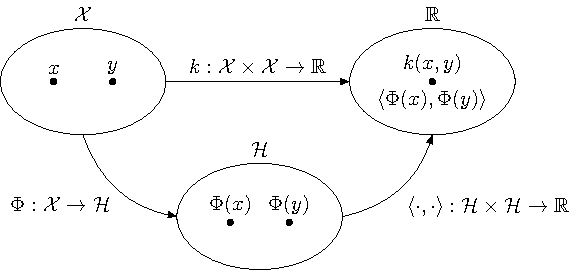
\includegraphics[]{figs/fig-kernel-map-diagram}
    \caption{Kernel map diagram.}
    \label{fig:kernel-map-diagram}
\end{figure}

Consider the feature map \(\Phi(x) = k(\cdot, x)\), for all \(x \in X\).
Taking the linear span of \(\Phi(X)\) gives us
\begin{equation}
    \lspan\{\Phi(x) : x \in X\}
    = \left\{
        f = \sum_{i=1}^{n} \alpha_i k( \cdot, x_i)
        \;\middle|\;
        n \in \NN, x_i \in X, \alpha_i \in \RR
    \right\},
\end{equation}
which forms a vector space.
Let \(f,g \in \lspan \Phi(X)\) such that
\begin{equation}
    \label{eqn:function-linear-combo}
    f = \sum_{i=1}^{n} \alpha_i k(\cdot, x_i)
    \quad\text{and}\quad
    g = \sum_{j=1}^{m} \beta_j k(\cdot, y_j).
\end{equation}
and define
\begin{equation}
    \label{eqn:pre-hilbert-inner-product}
    \langle f, g \rangle 
    = \sum_{i=1}^{n} \sum_{j=1}^{m} \alpha_i \beta_j k(x_i, y_j).
\end{equation}

Before we can prove that \Cref{eqn:pre-hilbert-inner-product} is an inner product, we need to show that \(k\) has the \textit{reproducing property}.
Let \(x \in X\).
Then by \Cref{eqn:function-linear-combo},
\begin{equation}
    \langle f, k(\cdot, x) \rangle = \sum_{i=1}^{n} \alpha k(x_i, x) = f(x).
\end{equation}

\begin{enumerate}
    \item Since \(k\) is symmetric, we have
    \begin{equation}
        \langle f, g \rangle
        = \sum_{i=1}^{n} \sum_{j=1}^{m} \alpha_i \beta_j k(x_i, y_j)
        = \sum_{j=1}^{m}\sum_{i=1}^{n}  \alpha_i \beta_j k(y_j, x_i)
        = \langle g, f \rangle.
    \end{equation}
    \item Using \Cref{eqn:function-linear-combo,eqn:pre-hilbert-inner-product}, we can write
    \begin{equation}
        \langle f, g \rangle
        = \sum_{i=1}^{n} \sum_{j=1}^{m} \alpha_i \beta_j k(x_i, y_j)
        = \sum_{j=1}^{m} \beta_j \sum_{i=1}^{n} \alpha_i k(x_i, y_j)
        = \sum_{j=1}^{m} \beta_j f(y_j).
    \end{equation}
    Then
    \begin{equation}
        \begin{aligned}[t]
            \langle f_1 + f_2, g \rangle
            &= \sum_{j=1}^{m} \beta_j \left[f_1(y_j) + f_2(y_j)\right]\\
            &= \sum_{j=1}^{m} \beta_j f_1(y_j) + \sum_{j=1}^{m} \beta_j f_2(y_j)\\
            &= \langle f_2, g \rangle + \langle f_1, g \rangle.
        \end{aligned}
    \end{equation}
    \item 
\end{enumerate}

% \subsubsection*{To do:}
% \begin{itemize}
%     \item move kernel/Gram matrix to its own definition
%     \item Define linear functionals
%     \item Define dual space (maybe?)
%     \item Riesz representation theorem
%     \item Define evaluation functionals
%     \item Define RKHS (continuous evaluation functionals)
%     \item An RKHS defines a unique reproducing kernel (by Riesz representation theorem).
%     \item Mercer's theorem.
%     \item A kernel defines a feature map.
%     \item A kernel defines a unique RKHS (by Mercer/Moore-Aronszajn).
%     \item We finally get \(k(x,y) = \langle \Phi(x), \Phi(y) \rangle_H\).
% \end{itemize}

\subsection{Constructing kernels}

\begin{theorem}
    \cite{rudin2020notes,shawe2004kernel}
    Suppose \(k_1\) and \(k_2\) are kernels over \(X \times X\).
    The following functions kernels.
    \begin{enumerate}
        \item \(k(x,y) = a_1 k_1(x,y) + a_2 k_2(x,y)\) for all \(a_1, a_2 \geq 0\).
        \item \(k(x,y) = k_1(x,y) k_2(x,y)\).
        \item \(k(x,y) = a_0 + a_1 k_1(x,y) + a_2 k_1(x,y)^2 + \cdots + a_n k_1(x,y)^n\) for all \(n \in \NN\) and \(a_0, \dots, a_n \geq 0\).
        \item \(k(x,y) = k_1(h(x),h(y))\) for all \(h : X \to X\).
        \item \(k(x,y) = g(x)g(y)\) for all \(g : X \to \RR\).
        \item \(k(x,y) = \exp(k_1(x,y))\).
    \end{enumerate}
\end{theorem}

\begin{proof}
    Let \(x_1, \dots, x_n \in X\) and \(c_1, \dots, c_n \in \RR\).
    \begin{enumerate}
        \item \label{itm:kernel-linear-combo}
        Let \(k = a_1k_1 + a_2k_2\) for \(a_1, a_2 \geq 0\).
        Since \(k_1\) and \(k_2\) are symmetric,
        \[
            k(x,y)
            = a_1k_1(x,y) + a_2k_2(x,y)
            = a_1k_1(y,x) + a_2k_2(y,x)
            = k(y,x),
        \]
        for all \(x,y \in X\).
        So, \(k\) is symmetric.

        Since \(k_1\) and \(k_2\) are positive semidefinite and \(a_1, a_2 \geq 0\),
        \begin{align*}
            \sum_{i=1}^{n} \sum_{j=1}^{n} c_i c_j k(x_i,x_j)
            &= \sum_{i=1}^{n} \sum_{j=1}^{n} c_i c_j (a_1 k_1(x_i,x_j) + a_2 k_2(x_i,x_j))\\
            &= a_1 \sum_{i=1}^{n} \sum_{j=1}^{n} c_i c_j k_1(x_i,x_j)
            + a_2 \sum_{i=1}^{n} \sum_{j=1}^{n} c_i c_j k_2(x_i,x_j)\\
            &\geq 0.
        \end{align*}
        So, \(k\) is positive semidefinite.
        \item \label{itm:kernel-product}
        Let \(k = k_1 k_2\).
        Define \(K\) so that \([K]_{ij} = k(x_i,x_j) = k_1(x_i, x_j) k_2(x_i, x_j)\).
        Let \(K_1\) and \(K_2\) be the Gram matrices for \(k_1\) and \(k_2\), respectively.
        Then \(K_1, K_2\) have orthonormal eigenvectors and nonnegative eigenvalues such that
        \def\dsum{\displaystyle\sum}
        \begin{align*}
            K_1 &= V LV^\top \\
            &= \begin{bmatrix}
                v_{11} & \cdots & v_{1n}\\
                \vdots & \ddots & \vdots\\
                v_{n1} & \cdots & v_{nn}\\
            \end{bmatrix}
            \begin{bmatrix}
                \lambda_{1} & \cdots & 0\\
                \vdots & \ddots & \vdots\\
                0 & \cdots & \lambda_{n}\\
            \end{bmatrix}
            \begin{bmatrix}
                v_{11} & \cdots & v_{n1}\\
                \vdots & \ddots & \vdots\\
                v_{1n} & \cdots & v_{nn}\\
            \end{bmatrix}\\
            &= \begin{bmatrix}
                \dsum_{j=1}^{n} \lambda_{j} v_{1j} v_{1j} & \cdots & \dsum_{j=1}^{n} \lambda_{j} v_{nj} v_{1j} \\
                \vdots & \ddots & \vdots\\
                \dsum_{j=1}^{n} \lambda_{j} v_{1j} v_{nj} & \cdots & \dsum_{j=1}^{n} \lambda_{j} v_{nj} v_{nj}\\
            \end{bmatrix}\\
            &= \sum_{j=1}^{n} \lambda_{j}
            \begin{bmatrix}
                v_{1j} v_{1j} & \cdots & v_{nj} v_{1j} \\
                \vdots & \ddots & \vdots\\
                v_{1j} v_{nj} & \cdots & v_{nj} v_{nj}\\
            \end{bmatrix}
            \intertext{and}
            K_2 &= UMU^\top = \sum_{j=1}^{n} \mu_{j}
            \begin{bmatrix}
                u_{1j} u_{1j} & \cdots & u_{nj} u_{1j} \\
                \vdots & \ddots & \vdots\\
                u_{1j} u_{nj} & \cdots & u_{nj} u_{nj}\\
            \end{bmatrix}.
        \end{align*}
        \def\v{\mathbf{v}}
        \def\u{\mathbf{u}}
        Let \(\v_i = \begin{bmatrix}
            v_{1i} & \cdots & v_{ni}
        \end{bmatrix}^\top\) and \(\u_j = \begin{bmatrix}
            u_{1j} & \cdots & u_{nj}
        \end{bmatrix}\), for all \(i,j = 1, 2, \dots, n\).
        Then
        \begin{align*}
            K &= K_1 \circ K_2\\
            &= \sum_{i=1}^{n} \lambda_{i}
            \begin{bmatrix}
                v_{1i} v_{1i} & \cdots & v_{ni} v_{1i} \\
                \vdots & \ddots & \vdots\\
                v_{1i} v_{ni} & \cdots & v_{ni} v_{ni}\\
            \end{bmatrix} \circ
            \sum_{j=1}^{n} \mu_{j}
            \begin{bmatrix}
                u_{1j} u_{1j} & \cdots & u_{nj} u_{1j} \\
                \vdots & \ddots & \vdots\\
                u_{1j} u_{nj} & \cdots & u_{nj} u_{nj}\\
            \end{bmatrix}\\
            &= \sum_{i=1}^{n} \sum_{j=1}^{n} \lambda_{i} \mu_{j}
            \begin{bmatrix}
                v_{1i} u_{1j} v_{1i} u_{1j} & \cdots & v_{1i} u_{1j} v_{ni} u_{nj} \\
                \vdots & \ddots & \vdots\\
                v_{ni} u_{nj} v_{1i} u_{1j} & \cdots & v_{ni} u_{nj} v_{ni}  u_{nj}
            \end{bmatrix}\\
            &= \sum_{i=1}^{n} \sum_{j=1}^{n} \lambda_{i} \mu_{j}
            \begin{bmatrix}
                v_{1i} u_{1j} \\ \vdots \\ v_{ni} u_{nj}
            \end{bmatrix}
            \begin{bmatrix}
                v_{1i} u_{1j} & \cdots & v_{ni} u_{nj}
            \end{bmatrix}\\
            &= \sum_{i=1}^{n} \sum_{j=1}^{n} \lambda_{i} \mu_{j}
            (\v_i \circ \u_j) (\v_i \circ \u_j)^\top,
        \end{align*}
        where \(\circ\) is the Hadamard product.
        Each \((\v_i \circ \u_j) (\v_i \circ \u_j)^\top\) is a symmetric positive semidefinite matrix.
        Since \(K_1, K_2\) are positive semidefinite, we have \(\lambda_i, \mu_i > 0\).
        Then \(K\) is symmetric positive semidefinite.
        \item By part \ref{itm:kernel-product}, \(k_1, k_1^2, \dots, k_1^n\) are kernels.
        By part \ref{itm:kernel-linear-combo}, \(a_0 + a_1 k_1 + a_2 k_1^2 + \dots + a_n k_1^n\) is a kernel.
        \item Since \(y_i = h(x_i) \in X\) for all \(i = 1,2,\dots, n\), we have
        \begin{align*}
            \sum_{i=1}^{n} \sum_{j=1}^{n} c_i c_j k(x_i,x_j)
            &= \sum_{i=1}^{n} \sum_{j=1}^{n} c_i c_j k_1(h(x_i), h(x_j))\\
            &= \sum_{i=1}^{n} \sum_{j=1}^{n} c_i c_j k_1(y_i, y_j)\\
            &\geq 0.
        \end{align*}
        \item Let \(g : X \to \RR\) and let \(c_i g(x_i) = y_i \in \RR\).
        If \(k(x,y) = g(x)g(y)\), then
        \begin{align*}
            \sum_{i=1}^{n} \sum_{j=1}^{n} c_i c_j k(x_i,x_j)
            &= \sum_{i=1}^{n} \sum_{j=1}^{n} c_i g(x_i) c_j g(x_j)\\
            &= \sum_{i=1}^{n} \sum_{j=1}^{n} y_i y_j\\
            % &= \sum_{\ell=1}^{n} \left(y_\ell^2 + \sum_{i=\ell+1}^{n} y_i y_\ell + \sum_{j=\ell+1}^{n} y_\ell y_j\right)\\
            % &= \sum_{i=1}^{n} \left(y_i^2 + 2\sum_{j=i+1}^{n} y_i y_j\right)\\
            &= \left(\sum_{i=1}^{n} y_i\right)^2\\
            &\geq 0.
        \end{align*}
        \item Let \(K_1\) be the Gram matrix for \(k_1\).
        If \(K_1 v = \lambda v\), then \(K_1^m = \lambda^m v\) for all \(m \in \NN\).
        So,
        \begin{align*}
            (\exp K_1) v
            = \sum_{m=0}^{\infty} \frac{K_1^m v}{m!}
            = \sum_{m=0}^{\infty} \frac{\lambda^m v}{m!}
            = e^\lambda v.
        \end{align*}
        Then \(K = \exp K_1\) has eigenvalues \(e^\lambda\).
        Since \(K_1\) is positive semidefinite, it has real eigenvalues so that \(e^\lambda > 0\).
        It follows that \(K\) is positive definite.
    \end{enumerate}
\end{proof}

\begin{theorem}[Gaussian kernel]
    \label{thm:gaussian-kernel}
    The function \(k : \RR^n \times \RR^n \to \RR\) defined by
    \[k(x,y) = \exp\left(\dfrac{-\|x-y\|^2_2}{\sigma^2}\right),\]
    is a kernel.
\end{theorem}

\begin{proof}
    
\end{proof}
\section{Kernel PCA}
Recall that linear PCA finds new components that reveal more information about the structure of high-dimensional data.
Since PCA is an orthogonal projection, the original data is rotated witin the original space of input variables.
The work of Sch\"olkopf, Smola, and M\"uller \cite{scholkopf1997kernel,scholkopf1998nonlinear} generalized PCA based on the successful application of kernel methods in support vector machines.
In kernel PCA, the inner product of the input space is replaced with the inner product of a feature space.
As such, the principal components of kernel PCA are nonlinear transformations of input variables, or features.

Using results from the previous section, a kernel function \(k\) defines a unique reproducing kernel Hilbert space \(H_k\) and feature map \(\Phi : X \to H_k\) such that
\begin{equation}
    \label{eqn:kernel-inner-product}
    k(x,y) = \langle \Phi(x), \Phi(y) \rangle,
\end{equation}
for all \(x, y \in H_k\).
By replacing the dot product in the formulation of the PCA algorithm, 

\subsection{Centering in the feature space}
Let \(\Phi : X \to H_k\) be a feature map determined by a kernel \(k\).
Since \(\Phi\) may be nonlinear, the image \(\Phi(x)\) of a centered vector \(x \in X\) is not guaranteed to be centered.
For an effective PCA algorithm, it is necessary to compute the Gram matrix of centered vectors in the feature space. \cite{scholkopf1998nonlinear}

Given \(x_1, \dots, x_m \in X\), the points
\begin{equation}
    \label{eqn:centered-features}
    \Phi_0(x_i) = \Phi(x_i) - \frac{1}{m} \sum_{i=1}^{m} \Phi(x_i), \quad \text{for \(i = 1,\dots,m\)}
\end{equation}
are the centered feature vectors in \(H_k\).
Then the centered Gram matrix becomes
\def\ipt#1{\left\langle #1 \right\rangle}
\begin{align*}
    [K_0]_{ij}
    &= \ipt{\Phi_0(x_i), \Phi_0(x_j)}\\
    &= \ipt{\Phi(x_i) - \frac{1}{m} \sum_{p=1}^{m} \Phi(x_p), \Phi(x_j) - \frac{1}{m} \sum_{q=1}^{m} \Phi(x_q)}\\
    &= \ipt{\Phi(x_i), \Phi(x_j)}
    \begin{aligned}[t]
        &- \frac{1}{m} \sum_{p=1}^{m} \ipt{\Phi(x_p), \Phi(x_j)}\\
        &- \frac{1}{m} \sum_{q=1}^{m} \ipt{\Phi(x_i), \Phi(x_q)}\\
        &+ \frac{1}{m^2} \sum_{p=1}^{m} \sum_{q=1}^{m} \ipt{\Phi(x_p), \Phi(x_q)}
    \end{aligned}\\
    &= k(x_i, x_j) - \frac{1}{m} \sum_{p=1}^{m} k(x_p, x_j) - \frac{1}{m} \sum_{q=1}^{m} k(x_i, x_q) + \frac{1}{m^2} \sum_{p=1}^{m} \sum_{q=1}^{m} k(x_p, x_q).
\end{align*}
If \(K\) is the uncentered Gram matrix, then the formula can be written as
\def\ones{\mathbf{1}_m}
\begin{equation}
    K_0 = K - \ones K - K \ones + \ones K \ones,
\end{equation}
where \(\ones\) is the \(m \times m\) matrix whose entries are \(1/m\).

\begin{example}
    Consider the problem of classifying points based on their radii.
    These points cannot be separated using a linear classifier in the two dimensions.
    However, by mapping them to a three-dimensional space, they can be separated by planes.
    Applying kernel PCA, these points can be sent to the RKHS associated with a Gaussian kernel without using an explicit feature map.
    The points in this high-dimensional feature space can then be projected onto the first three principal components to find separation boundaries.
    See \Cref{fig:gaussian-kpca-example}.
    \begin{figure}
        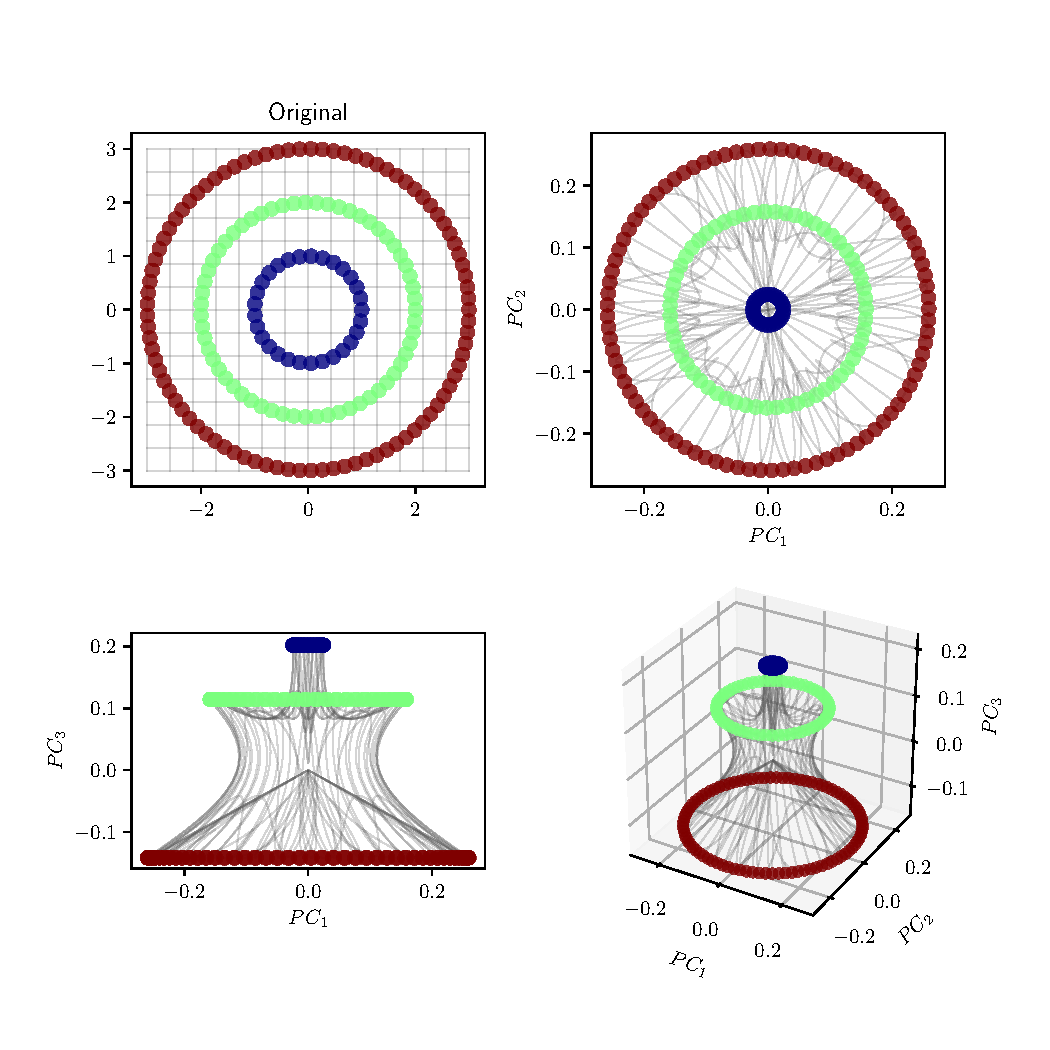
\includegraphics[width=\textwidth]{figs/fig_kpca_example.pdf}
        \caption{An idealized set of points in the plane are classified based on their radius. Kernel PCA with the Gaussian kernel is applied to find separation boundaries using the first three principal components.}
        \label{fig:gaussian-kpca-example}
    \end{figure}
\end{example}

% To do:
% - more about feature maps
% - use encode paper, kpca section for feature map/ feature space
% - nonlinear maps
% - rkhs
% - kpca algorithm
% - example
\section{Conclusion}
Kernel PCA is a powerful tool that reveals nonlinear patterns in data.
This is only one example of an entire class of kernel methods that extend the capabilities of linear algorithms.
By exploring the theory behind kernel methods, we see how much structure exists due to symmetric positive semidefinite kernels.
\appendix
\section{Linear Algebra}
A number of matrix definitions and results are presented without proof.
These can be found in \cite{horn2013matrix}.


\begin{enumerate}
    \item A square matrix \(A\) is \textit{normal} if \(AA^\top = A^\top A\).
    \item Symmetric matrices are normal.
    \item Symmetric matrices have orthogonal eigenvectors and real eigenvectors.
    \item Positive semidefinite matrices have nonnegative eigenvalues.
    \item \(A\) is positive semidefinite if and only if there exists a matrix \(B\) such that \(A = B^\top B\). We say \(B\) is the \textit{square root} of \(A\) and write \(A^{1/2} = B\).
    \item Positive definite matrices have positive eigenvalues.
    \item \(A^\top A\) and \(AA^\top\) are symmetric positive semi-definite.
\end{enumerate}

\begin{lemma}
    \label{lem:spsd-factorization}
    Let \(A\) be a positive semidefinite matrix.
    Then \(A\) has the factorization \(A = B^\top B\).
    We call \(\)
\end{lemma}
\begin{proof}
    Since \(A\) is symmetric, it is diagonalizable and we can write \(A = V^\top D V\).
    Since \(A\) is positive semidefinite, 
\end{proof}

\subsection{Matrix operations and notation}
\label{subsec:matrix-operations}

Let \(A\) be an \(n \times d\) matrix.
We write \([A]_{ij}\) to indicate the matrix entry in the \(i\)-th row and the \(j\)-th column.

\begin{definition}
    Define the \textit{entry-wise mean} of \(A\) as
    \begin{equation}
        \label{eqn:matrix-mean}
        \mean(A) = \frac{1}{nd} \sum_{i=1}^{n} \sum_{j=1}^{d} [A]_{ij}.
    \end{equation}
    Define the \textit{column-wise mean} of \(A\) as a \(1 \times d\) row vector whose \(j\)-th entry is the mean of column \(j\) given by the formula
    \begin{equation}
        \label{eqn:column-mean}
        \begin{aligned}
            \colmean(A)
            &= \begin{bmatrix}
                \rule[-.5em]{0em}{1em}
                \frac{1}{n} \sum_{i=1}^{n} [A]_{i1}, &
                \frac{1}{n} \sum_{i=1}^{n} [A]_{i2}, &
                \dots, &
                \frac{1}{n} \sum_{i=1}^{n} [A]_{id}
            \end{bmatrix}\\
            &= \frac{1}{n} \sum_{i=1}^{n} \begin{bmatrix}
                \rule[-.5em]{0em}{1em}
                [A]_{i1}, &
                [A]_{i2}, &
                \dots, &
                [A]_{id}
            \end{bmatrix}.
        \end{aligned}
    \end{equation}
    Define the \textit{row-wise mean} of \(A\) as an \(n \times 1\) column vector whose \(i\)-th entry is the mean of row \(i\) given by the formula
    \begin{equation}
        \label{eqn:row-mean}
        \rowmean(A) = \begin{bmatrix}
            \rule{0em}{1.5em}
            \frac{1}{d} \sum_{j=1}^{d} [A]_{1j} \\
            \rule{0em}{2em}
            \frac{1}{d} \sum_{j=1}^{d} [A]_{2j} \\
            \vdots \\
            \rule[-.7em]{0em}{2em}
            \frac{1}{d} \sum_{j=1}^{d} [A]_{nj}
        \end{bmatrix}
        = \frac{1}{d} \sum_{j=1}^{d} \begin{bmatrix}
            [A]_{1j}\\
            [A]_{2j}\\
            \vdots \\
            [A]_{nj}\\
        \end{bmatrix}.
    \end{equation}
\end{definition}

\def\repmat#1#2{\textstyle\left[#1\right]_{#2}}
Let \([a]_{p \times q}\) denote the \(p \times q\) repeated matrix whose entries are all \(a\).
Then \cref{eqn:matrix-mean,eqn:column-mean,eqn:row-mean} can be written as
\begin{align}
    \mean(A) &= \repmat{\frac{1}{n}}{1 \times n} \cdot A \cdot \repmat{\frac{1}{d}}{d \times 1}\\
    \colmean(A) &= \repmat{\frac{1}{n}}{1 \times d} \cdot A \\
    \rowmean(A) &= A \cdot \repmat{\frac{1}{d}}{d \times 1}.
\end{align}

% \begin{definition}
%     \def\a{\mathbf{a}}
%     Let \(A\) be an \(n \times d\) matrix whose columns \(\a_1, \a_2,\dots,\a_d \in \RR^n\) represent variables and rows represent observations.
%     Then the \textit{covariance matrix} of \(A\) is given by
%     \begin{equation}
%         \label{eqn:covariance-matrix}
%         \cov(A) = \begin{bmatrix}
%             \cov(\a_1, \a_1) & \cov(\a_1, \a_2) & \cdots & \cov(\a_1, \a_d)\\
%             \cov(\a_2, \a_1) & \cov(\a_2, \a_2) & \cdots & \cov(\a_2, \a_d)\\
%             \vdots & \vdots & \ddots & \vdots\\
%             \cov(\a_d, \a_1) & \cov(\a_d, \a_2) & \cdots & \cov(\a_d, \a_d)\\
%         \end{bmatrix}.
%     \end{equation}
%     If \(A\) is centered, i.e., the columns all have mean zero, then we can write
%     \begin{equation}
%         \label{eqn:centered-covariance-matrix}
%         \cov(A) = \frac{1}{n-1}A^\top A.
%     \end{equation}
%     % Here, \(1/(m-1)\) is due to Bessel's correction.
%     % https://en.wikipedia.org/wiki/Bessel%27s_correction
% \end{definition}

\subsection{Broadcasting}
\label{subsec:broadcasting}

\def\b{\mathbf{b}}
Consider the sum of two real matrices \(A + B\).
By definition, \(A\) and \(B\) must both have size \(n \times d\).
This means we cannot add a \(2 \times 3\) matrix \(A\) and a \(2 \times 1\) vector \(\b\).
However, in many programming languages the sum \(A + \b\) would be handled using \textit{broadcasting} \cite{harris2020array}.
In this case, \(\b\) is converted to a \(2 \times 3\) matrix \(\begin{bmatrix} \b & \b & \b \end{bmatrix}\) so that normal matrix addition applies.
Generally, broadcasting a vector \(\b \in \RR^n\) to an \(n \times d\) matrix can be represented as the matrix product
\begin{equation}
    \label{eqn:vector-broadcasting}
    \b \cdot [1]_{1 \times d}
    = \begin{bmatrix}
        b_1 \\ b_2 \\ \vdots \\ b_n
    \end{bmatrix}
    \cdot
    \begin{bmatrix}
        1 & 1 & \cdots & 1
    \end{bmatrix}
    = \begin{bmatrix}
        b_1 & b_1 & \cdots & b_1 \\
        b_2 & b_2 & \cdots & b_2 \\
        \vdots & \vdots & & \vdots \\
        b_n & b_n & \cdots & b_n
    \end{bmatrix},
\end{equation}
where the notation \([a]_{n \times d}\) represents an \(n \times d\) matrix whose entries are all \(a\).
\begin{definition}
    \label{def:broadcast-addition}
    For an \(n \times d\) matrix \(A\), we can define addition by an \(n \times 1\) column vector \(\mathbf{c}\) as
    \begin{equation}
        \label{eqn:matrix-col-vector-addition}
        A + \mathbf{c} := A + \mathbf{c} \cdot [1]_{1 \times d}.
    \end{equation}
    Similarly, addition by a \(1 \times d\) row vector \(\mathbf{r}\) can be defined as
    \begin{equation}
        \label{eqn:matrix-row-vector-addition}
        A + \mathbf{r} := A + [1]_{n \times 1} \cdot \mathbf{r}
    \end{equation}
    and addition by a scalar \(a\) can be defined as
    \begin{equation}
        \label{eqn:matrix-scalar-addition}
        A + a := A + a \cdot [1]_{n \times d}.
    \end{equation}
\end{definition}

The left hand sides of \cref{eqn:matrix-col-vector-addition,eqn:matrix-row-vector-addition,eqn:matrix-scalar-addition} are more concise and intuitive than the right hand sides.
Provided that the vector types are clearly defined and compatible, there should be no ambiguity when adding column vectors, row vectors, and scalars to matrices.
Moreover, this method of broadcasting is consistent with scientific programming languages.
\section{Riesz Representation Theorem}
\begin{theorem}[Riesz Representation Theorem]
    \cite{small1994hilbert} % page 22
    Let \(\phi : H \to \RR\) be a continuous linear functional defined on a Hilbert space \(\H\).
    Then there exists a unique element \(g \in \H\) such that \(\phi(g) = \langle f, g \rangle_H\) for all \(g \in \H\).
\end{theorem}

\begin{proof}
    
\end{proof}

% To do
% - linear functionals
% - construct RKHS
\section{Mercer's Theorem}
% To do
% - mercer kernel
\section{Code}
% TODO: Add code
\lstinputlisting[
    language=Python,
    caption=PCA example,
    label=lst:pca-example
]{../py/pca-example.py}
\lstinputlisting[
    language=Python,
    caption=PCA source functions,
    label=lst:pca-source
]{../py/pca.py}


\nocite{*}
\bibliographystyle{plain}
\bibliography{refs}
\end{document}